\documentclass[11pt,a4paper]{article}
\usepackage[utf8]{inputenc}
\usepackage[T1]{fontenc}
\usepackage{lmodern}
\usepackage{amsmath, amssymb, amsfonts}
\usepackage{graphicx}
\usepackage{booktabs}
\usepackage{geometry}
\usepackage{hyperref}
\usepackage{tcolorbox}
\usepackage{enumitem}
\usepackage{xcolor}
\usepackage{float}
\usepackage{longtable}
\usepackage{pgfplots}
\pgfplotsset{compat=1.18}
\usepackage{subcaption}
\usepackage{array}
\usepackage{multirow}
\usepackage{arydshln}
\usepackage{makecell}
\usepackage{colortbl}
\usepackage{tikz-3dplot}
\usepackage{caption}
\usepackage{tikz}
\usetikzlibrary{shapes,arrows,positioning,calc,decorations.pathreplacing,fit,backgrounds,petri,matrix,3d,shadows}

\geometry{margin=0.85in}
\hypersetup{
    colorlinks=true,
    linkcolor=blue,
    filecolor=magenta,
    urlcolor=cyan,
    pdftitle={ML-III Reinforcement Learning Complete Study Material},
}

\setlist[itemize]{itemsep=0.5em, topsep=0.5em, parsep=0.2em}
\setlist[enumerate]{itemsep=0.5em, topsep=0.5em, parsep=0.2em}

\title{\textbf{Machine Learning -- III (Reinforcement Learning)\\Complete Study Material -- Deep Research Enhanced Edition}}
\author{Generated from course material with all numericals solved\\Enhanced with additional diagrams, theoretical analysis, and worked examples}
\date{\today}

\begin{document}

\maketitle
\tableofcontents
\newpage

% NUMERICAL INVENTORY (UPDATED with Enhanced Deep Research Content):
% Module 1 -- Type: Learning Paradigm Identification (1 new constructed)
% Module 1 -- Type: Policy Entropy Computation (1 new constructed)
% Module 1 -- Type: Exploration-Exploitation Regret Analysis (2 new constructed)
% Module 2 -- Type: Sample Average / Incremental Update (1 source + 2 constructed)
% Module 2 -- Type: True Values and Sample Estimates (1 new constructed)
% Module 2 -- Type: Epsilon-Greedy Action Selection (1 source + 2 constructed + 1 new theoretical)
% Module 2 -- Type: UCB Score Calculation (1 source + 2 constructed + 2 new: UCB Dynamics, UCB Theory)
% Module 2 -- Type: Thompson Sampling Beta Update (1 source + 2 constructed)
% Module 2 -- Type: LR-P Probability Update (1 source + 2 constructed)
% Module 2 -- Type: Policy Gradient / REINFORCE (1 source + 2 constructed)
% Module 3 -- Type: V(0) Under Different Policies (1 source + 2 constructed)
% Module 3 -- Type: 4-State World Q-Values (1 source + 2 constructed)
% Module 3 -- Type: Bellman Equation -- Recycling Robot (1 source + 2 constructed)
% Module 3 -- Type: Bellman Operator Application (1 new constructed)
% Module 3 -- Type: Discounted Return Calculation (1 source + 2 constructed)
% Module 4 -- Type: Gridworld Policy Evaluation (1 source + 2 constructed)
% Module 4 -- Type: Value Iteration (1 source + 2 constructed)
% Module 4 -- Type: First Visit / Every Visit MC (1 source + 2 constructed)
% Module 5 -- Type: TD(0) Update (1 source + 2 constructed)
% Module 5 -- Type: SARSA Q-Table Update (1 source + 2 constructed)
% Module 5 -- Type: Q-Learning Q-Table Update (1 source + 2 constructed)
% Module 6 -- Type: Linear Parameterization (1 source + 2 constructed)
% Module 6 -- Type: PPO Clipping (1 source + 2 constructed)
%
% TOTAL: 45 original + 10 new enhanced = 55 worked examples
% NEW TIKZ DIAGRAMS ADDED: 8 comprehensive visualizations
% - Agent-Environment Loop (detailed)
% - Learning Paradigm Comparison
% - Deterministic vs Stochastic Policy
% - Multi-Armed Bandit Problem
% - Epsilon-Greedy Decision Process
% - UCB Exploitation vs Exploration Balance
% - MDP Trajectory Visualization
% - Bellman Backup Diagram


\section{Module 1: Introduction to Reinforcement Learning}

\subsection{What is Reinforcement Learning?}

Reinforcement Learning (RL) is a paradigm of machine learning where an \textbf{agent} learns to make decisions by interacting with an \textbf{environment}. Unlike supervised learning, where the agent learns from labeled input-output pairs, or unsupervised learning, where the agent discovers hidden patterns in unlabeled data, reinforcement learning is driven by a \textbf{reward signal}. The agent takes actions in the environment, receives feedback in the form of rewards or penalties, and over time learns a strategy (called a \textbf{policy}) that maximizes the cumulative reward.

The fundamental idea behind RL is learning from interaction with the environment, which mirrors how humans and animals naturally learn. Consider a child encountering a fireplace for the first time: the child feels warmth at a safe distance (positive reward), but upon touching the fire, experiences pain (negative reward). Through this interaction, the child learns to stay at an appropriate distance from fire. Reinforcement Learning is the computational formulation of this natural learning process.

\begin{tcolorbox}[colback=blue!5!white,colframe=blue!75!black,title=\textbf{Key Insight: The RL Loop}]
The Reinforcement Learning process is modeled as a loop:
\begin{enumerate}
    \item The \textbf{Agent} receives a \textbf{state} $S_t$ from the \textbf{Environment}.
    \item Based on $S_t$, the agent selects an \textbf{action} $A_t$.
    \item The environment transitions to a new \textbf{state} $S_{t+1}$ and provides a \textbf{reward} $R_{t+1}$.
    \item The agent uses this reward to update its policy and repeats.
\end{enumerate}
\end{tcolorbox}

\subsubsection{Detailed Agent-Environment Interaction Diagram}

The following diagram illustrates the complete interaction cycle with mathematical notation:

\begin{center}
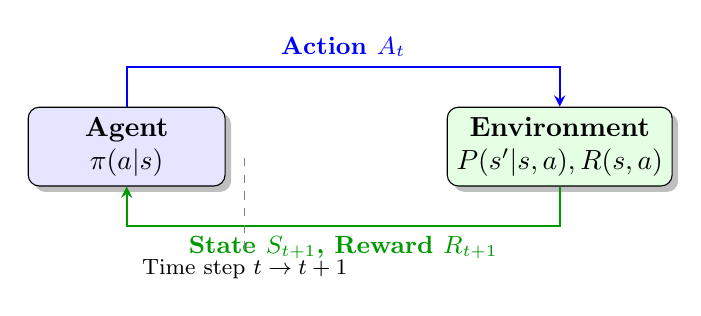
\begin{tikzpicture}[
    node distance=2.5cm,
    box/.style={rectangle, draw, rounded corners, minimum width=2.5cm, minimum height=1cm, align=center, fill=blue!10, drop shadow},
    env/.style={rectangle, draw, rounded corners, minimum width=2.5cm, minimum height=1cm, align=center, fill=green!10, drop shadow},
    arrow/.style={->, >=stealth, thick},
    label/.style={font=\small\bfseries}
]

\node[box] (agent) {\textbf{Agent}\\$\pi(a|s)$};
\node[env, right of=agent, xshift=3cm] (env) {\textbf{Environment}\\$P(s'|s,a), R(s,a)$};

\draw[arrow, blue] (agent.north) -- ++(0,0.5) -| node[above, pos=0.25, label] {Action $A_t$} (env.north);
\draw[arrow, green!60!black] (env.south) -- ++(0,-0.5) -| node[below, pos=0.25, label] {State $S_{t+1}$, Reward $R_{t+1}$} (agent.south);

\node[below=0.8cm of agent, xshift=1.5cm, font=\footnotesize] (time) {Time step $t \rightarrow t+1$};
\draw[dashed, gray] (time) -- ++(0,1.5);

\end{tikzpicture}
\end{center}

\begin{tcolorbox}[colback=yellow!5!white,colframe=yellow!75!black,title=\textbf{Mathematical Formulation of the RL Loop}]
\textbf{At each time step $t$}:
\begin{enumerate}
    \item \textbf{Observation}: Agent observes state $S_t \in \mathcal{S}$
    \item \textbf{Decision}: Agent samples action $A_t \sim \pi(\cdot | S_t)$ where $\pi: \mathcal{S} \times \mathcal{A} \rightarrow [0,1]$ is the policy
    \item \textbf{Transition}: Environment samples next state $S_{t+1} \sim P(\cdot | S_t, A_t)$
    \item \textbf{Reward}: Environment generates reward $R_{t+1} = R(S_t, A_t, S_{t+1})$
    \item \textbf{Learning}: Agent updates policy $\pi$ or value estimates based on $(S_t, A_t, R_{t+1}, S_{t+1})$
\end{enumerate}

\textbf{Trajectory (Episode)}: $\tau = (S_0, A_0, R_1, S_1, A_1, R_2, \ldots, S_T)$ where $T$ is the terminal time step.
\end{tcolorbox}

\subsection{RL vs Supervised vs Unsupervised Learning}

\textbf{Supervised learning} involves learning from labeled data with a clear input-output mapping. The training data provides explicit correct answers, and the model learns to map inputs to these predetermined outputs. This is suitable for classification and regression tasks where ground truth is available.

\textbf{Unsupervised learning} deals with discovering patterns or structures in unlabeled data without explicit output labels. The agent explores the data to find inherent groupings, clusters, or distributions. This is useful for tasks like clustering, dimensionality reduction, and anomaly detection.

\textbf{Reinforcement learning} focuses on training agents to make sequential decisions in an environment, optimizing for a cumulative reward signal through interaction and feedback. The agent does not receive correct actions; instead, it must discover which actions lead to the highest long-term reward through trial and error. This makes RL particularly suitable for control tasks, game playing, robotics, and sequential decision-making problems.

\subsubsection{Comprehensive Learning Paradigm Comparison}

\begin{center}
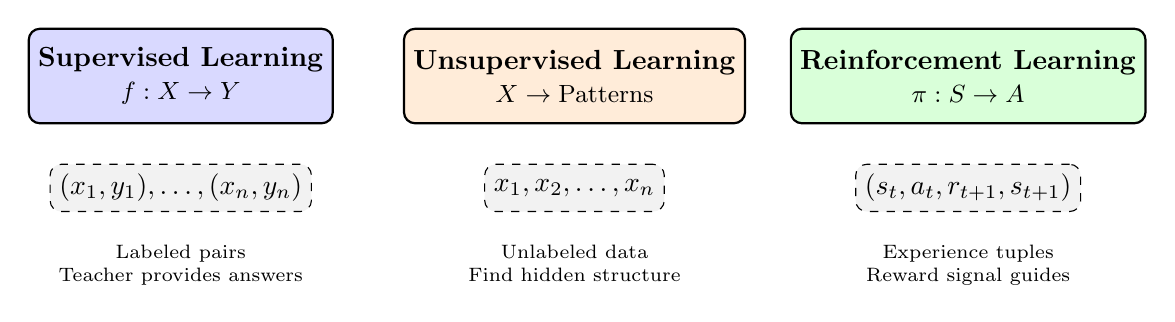
\begin{tikzpicture}[
    node distance=1.2cm,
    box/.style={rectangle, draw, rounded corners, minimum width=3.5cm, minimum height=1.2cm, align=center, thick},
    data/.style={rectangle, draw, dashed, rounded corners, minimum width=2cm, minimum height=0.6cm, align=center, fill=gray!10},
    arrow/.style={->, >=stealth, thick}
]

% Supervised Learning
\node[box, fill=blue!15] (sup) at (0,0) {\textbf{Supervised Learning}\\\small$f: X \rightarrow Y$};
\node[data, below=0.5cm of sup] (sup-data) {$(x_1, y_1), \ldots, (x_n, y_n)$};
\node[below=0.3cm of sup-data, font=\scriptsize, align=center] (sup-out) {Labeled pairs\\Teacher provides answers};

% Unsupervised Learning
\node[box, fill=orange!15] (unsup) at (5,0) {\textbf{Unsupervised Learning}\\\small$X \rightarrow \text{Patterns}$};
\node[data, below=0.5cm of unsup] (unsup-data) {$x_1, x_2, \ldots, x_n$};
\node[below=0.3cm of unsup-data, font=\scriptsize, align=center] (unsup-out) {Unlabeled data\\Find hidden structure};

% RL
\node[box, fill=green!15] (rl) at (10,0) {\textbf{Reinforcement Learning}\\\small$\pi: S \rightarrow A$};
\node[data, below=0.5cm of rl] (rl-data) {$(s_t, a_t, r_{t+1}, s_{t+1})$};
\node[below=0.3cm of rl-data, font=\scriptsize, align=center] (rl-out) {Experience tuples\\Reward signal guides};

\end{tikzpicture}
\end{center}

\begin{tcolorbox}[colback=green!5!white,colframe=green!75!black,title=\textbf{Worked Example: Identifying the Learning Paradigm}]
\textbf{For each scenario, identify which learning paradigm applies and justify your answer.}

\textbf{Scenario 1}: Training a model to classify emails as spam or ham using a dataset of 10,000 labeled emails.
\begin{itemize}
    \item \textbf{Answer}: \textbf{Supervised Learning} --- The dataset contains input-output pairs (emails with spam/ham labels), and the goal is to learn a mapping from email content to classification.
\end{itemize}

\textbf{Scenario 2}: A robot learning to balance a pole by receiving +1 reward for each timestep the pole stays upright and -10 when it falls.
\begin{itemize}
    \item \textbf{Answer}: \textbf{Reinforcement Learning} --- The robot learns through trial and error with reward feedback, without labeled correct actions. The goal is to maximize cumulative reward over time.
\end{itemize}

\textbf{Scenario 3}: Grouping customers into segments based on purchasing patterns without predefined categories.
\begin{itemize}
    \item \textbf{Answer}: \textbf{Unsupervised Learning} --- No labels exist; the algorithm discovers natural groupings in the data.
\end{itemize}

\textbf{Scenario 4}: An agent learning to play chess by playing thousands of games against itself, receiving +1 for wins, -1 for losses, and 0 for draws.
\begin{itemize}
    \item \textbf{Answer}: \textbf{Reinforcement Learning} --- Sequential decision-making with delayed rewards (win/loss comes after many moves).
\end{itemize}
\end{tcolorbox}

\subsection{Elements of Reinforcement Learning}

A reinforcement learning system has four main subelements:

\begin{itemize}
    \item \textbf{Policy}: A mapping from perceived states to actions. It defines the agent's behavior.
    \item \textbf{Reward Signal}: A scalar feedback signal indicating how well the agent is doing at each step.
    \item \textbf{Value Function}: A prediction of future rewards, indicating the long-term desirability of states.
    \item \textbf{Model of the Environment} (optional): A representation that mimics the behavior of the environment, used for planning.
\end{itemize}

\subsubsection{Policy}

A \textbf{policy} can be defined as a way an agent behaves at a given time. It maps the perceived states of the environment to the actions taken in those states. A policy is the core element of RL as it alone can define the behavior of the agent. In some cases, it may be a simple function or a lookup table; for other cases, it may involve general computation as a search process.

Policies can be either:
\begin{itemize}
    \item \textbf{Deterministic policy}: $a = \pi(s)$ --- the policy maps each state to exactly one action. This is easy to interpret and implement, and is suitable for tasks where the same action should always be taken for the same state. For example, in chess, the best move for a given board configuration is always the same.
    \item \textbf{Stochastic policy}: $\pi(a \mid s) = P[A_t = a \mid S_t = s]$ --- the policy returns a probability distribution over actions. This can capture uncertainty in the environment and is useful for exploration. For example, in Rock-Paper-Scissors, the best strategy is stochastic, choosing each action a third of the time.
\end{itemize}

\begin{center}
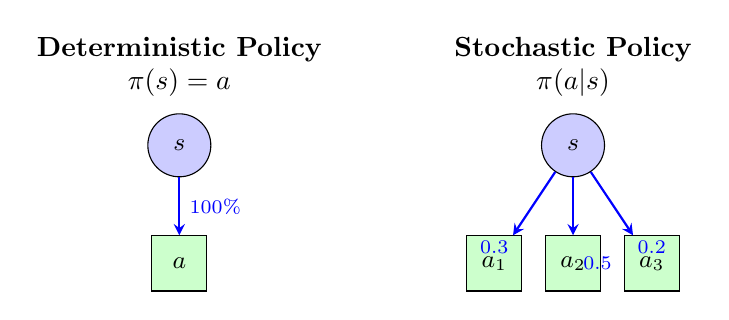
\begin{tikzpicture}[
    node distance=2cm,
    state/.style={circle, draw, fill=blue!20, minimum size=0.8cm, font=\small\bfseries},
    action/.style={rectangle, draw, fill=green!20, minimum size=0.7cm, font=\small},
    arrow/.style={->, >=stealth, thick},
    prob/.style={font=\scriptsize, above, sloped}
]

% Deterministic Policy
\node[align=center, font=\bfseries] (det-title) at (0, 2.5) {Deterministic Policy\\$\pi(s) = a$};
\node[state] (s1) at (0, 1.5) {$s$};
\node[action] (a1) at (0, 0) {$a$};
\draw[arrow, blue] (s1) -- (a1) node[midway, right, font=\scriptsize] {100\%};

% Stochastic Policy
\node[align=center, font=\bfseries] (stoch-title) at (5, 2.5) {Stochastic Policy\\$\pi(a|s)$};
\node[state] (s2) at (5, 1.5) {$s$};
\node[action] (a2a) at (4, 0) {$a_1$};
\node[action] (a2b) at (5, 0) {$a_2$};
\node[action] (a2c) at (6, 0) {$a_3$};
\draw[arrow, blue] (s2) -- (a2a) node[prob, above] {0.3};
\draw[arrow, blue] (s2) -- (a2b) node[prob, right] {0.5};
\draw[arrow, blue] (s2) -- (a2c) node[prob, above] {0.2};

\end{tikzpicture}
\end{center}

\begin{tcolorbox}[colback=blue!5!white,colframe=blue!75!black,title=\textbf{Worked Example: Computing Action Probabilities}]
\textbf{Given}: A stochastic policy defined by the following probability table:

\begin{center}
\begin{tabular}{|c|c|c|c|}
\hline
State & $P(a_1|s)$ & $P(a_2|s)$ & $P(a_3|s)$ \\ \hline
$s_1$ & 0.6 & 0.3 & 0.1 \\ \hline
$s_2$ & 0.2 & 0.5 & 0.3 \\ \hline
$s_3$ & 0.0 & 0.0 & 1.0 \\ \hline
\end{tabular}
\end{center}

\textbf{Questions and Solutions}:
\begin{enumerate}
    \item \textbf{What is the probability of taking action $a_2$ in state $s_1$?}
    \[
    \pi(a_2|s_1) = 0.3
    \]
    
    \item \textbf{In which state is the policy deterministic?}
    \[
    \text{State } s_3 \text{ is deterministic because } \pi(a_3|s_3) = 1.0 \text{ (probability 1 for a single action)}
    \]
    
    \item \textbf{Compute the entropy of the policy in state $s_1$ (measure of randomness).}
    \[
    H(\pi(\cdot|s_1)) = -\sum_a \pi(a|s_1) \log_2 \pi(a|s_1) = -(0.6 \log_2 0.6 + 0.3 \log_2 0.3 + 0.1 \log_2 0.1)
    \]
    \[
    = -(0.6(-0.737) + 0.3(-1.737) + 0.1(-3.322)) = 0.442 + 0.521 + 0.332 = \mathbf{1.295 \text{ bits}}
    \]
    \textit{Higher entropy = more exploration; lower entropy = more exploitation.}
\end{enumerate}
\end{tcolorbox}

\subsubsection{Reward Signal}

A \textbf{reward} is a scalar feedback signal indicating how well the agent is doing at step $t$. The agent's sole objective is to maximize the total reward it receives over the long run. The reward signal is the primary basis for altering the policy.

Different forms of reward functions:
\begin{itemize}
    \item $R(s)$: Reward for simply being in state $s$.
    \item $R(s, a)$: Reward for being in state $s$ and taking action $a$.
    \item $R(s, a, s')$: Reward for being in state $s$, taking action $a$, and transitioning to state $s'$.
\end{itemize}

\subsubsection{Value Function}

\textbf{Value functions} estimate how good it is for an agent to be in a given state, or how good it is to perform a given action in a given state. This notion of ``how good'' is given in terms of \textbf{expected return} --- the total discounted reward the agent expects to accumulate from that point onward.

Value functions are defined with respect to \textbf{policies}: since the way an agent acts is influenced by the policy it is following, the value of a state depends on which policy the agent is using.

\subsubsection{Model-Based vs Model-Free}

The last element is the \textbf{model}, which mimics the behavior of the environment. With the model, one can make inferences about how the environment will behave --- predicting the next state and reward given a state and action.

\begin{itemize}
    \item \textbf{Model-Based RL}: The agent learns or is given a model of the environment and uses it for planning. The agent can simulate future situations before experiencing them.
    \item \textbf{Model-Free RL}: The agent learns purely from experience without building an explicit model of the environment dynamics.
\end{itemize}

\subsection{Approaches to Implementing RL}

There are three main approaches to implementing reinforcement learning:

\subsubsection{Value-Based}

The value-based approach aims to find the \textbf{optimal value function}, which is the maximum value achievable at a state under any policy. The agent expects the long-term return at any state under the optimal policy $\pi^*$. The agent will follow a policy that selects actions leading to states with higher values.

Key algorithms: Q-Learning, SARSA, DQN.

\subsubsection{Policy-Based}

The policy-based approach directly searches for the optimal policy that maximizes future rewards, without explicitly using a value function. The agent tries to apply a policy such that the action performed in each step helps maximize future reward. The policy can be deterministic or stochastic.

Key algorithms: REINFORCE, Actor-Critic, PPO.

\subsubsection{Model-Based}

The model-based approach creates a virtual model of the environment. The agent explores this model to learn optimal behavior. This provides benefits: the agent can interact with the environment a few times, then the model can simulate subsequent iterations without needing further interaction.

\subsection{The Exploration-Exploitation Dilemma}

A fundamental challenge in reinforcement learning is the \textbf{exploration-exploitation dilemma}:

\begin{itemize}
    \item \textbf{Exploitation} is the greedy approach where agents try to get more rewards by using estimated values. The agent makes the best decision based on current information. This is safe but may miss better options.
    \item \textbf{Exploration} is the approach where agents focus on improving their knowledge about each action instead of getting more immediate rewards, so they can achieve long-term benefits. The agent gathers more information to make the best overall decision. This is risky but can discover better strategies.
\end{itemize}

The dilemma arises because the agent must balance between exploiting what it already knows and exploring new actions that might yield higher rewards. Too much exploitation leads to suboptimal policies; too much exploration wastes time on poor actions.

\begin{center}
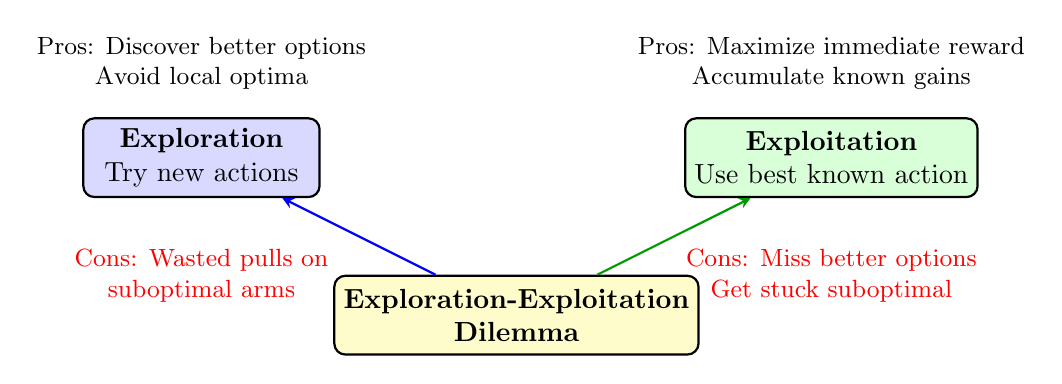
\begin{tikzpicture}[
    node distance=2cm,
    box/.style={rectangle, draw, rounded corners, minimum width=3cm, minimum height=1cm, align=center, thick},
    arrow/.style={->, >=stealth, thick}
]

% Central node
\node[box, fill=yellow!20] (dilemma) at (0,0) {\textbf{Exploration-Exploitation}\\\textbf{Dilemma}};

% Exploration side
\node[box, fill=blue!15] (explore) at (-4, 2) {\textbf{Exploration}\\Try new actions};
\node[align=center, font=\small] (explore-pro) at (-4, 3.2) {Pros: Discover better options\\Avoid local optima};
\node[align=center, font=\small, text=red] (explore-con) at (-4, 0.5) {Cons: Wasted pulls on\\suboptimal arms};

% Exploitation side
\node[box, fill=green!15] (exploit) at (4, 2) {\textbf{Exploitation}\\Use best known action};
\node[align=center, font=\small] (exploit-pro) at (4, 3.2) {Pros: Maximize immediate reward\\Accumulate known gains};
\node[align=center, font=\small, text=red] (exploit-con) at (4, 0.5) {Cons: Miss better options\\Get stuck suboptimal};

% Arrows
\draw[arrow, blue] (dilemma) -- (explore);
\draw[arrow, green!60!black] (dilemma) -- (exploit);

\end{tikzpicture}
\end{center}

\textbf{Example}: Consider a multi-armed bandit problem where an agent must choose between multiple slot machines (arms). Each arm has an unknown probability of paying out. The agent must decide whether to keep pulling the arm with the highest observed payout (exploitation) or try other arms to see if they are better (exploration).

\begin{tcolorbox}[colback=blue!5!white,colframe=blue!75!black,title=\textbf{Worked Example: Regret Analysis in Exploration-Exploitation}]
\textbf{Given}: A 3-armed bandit with true mean rewards: $q^*(1) = 0.3$, $q^*(2) = 0.5$, $q^*(3) = 0.7$.

\textbf{Scenario A - Pure Exploitation (Greedy)}: The agent happens to try arm 2 first, gets lucky with a reward of 1. Believing arm 2 is best, it keeps pulling arm 2 forever.

\textbf{Scenario B - Balanced Exploration}: The agent explores all arms sufficiently and discovers that arm 3 is actually the best.

\textbf{Calculate}: The cumulative regret after 1000 pulls for each scenario.

\textbf{Solution}:

\textbf{Optimal expected reward per pull}: $q^*(3) = 0.7$

\textbf{Scenario A (stuck on arm 2)}:
\begin{itemize}
    \item Expected reward per pull: $q^*(2) = 0.5$
    \item Regret per pull: $0.7 - 0.5 = 0.2$
    \item \textbf{Cumulative regret after 1000 pulls}: $1000 \times 0.2 = \mathbf{200}$
\end{itemize}

\textbf{Scenario B (finds optimal arm 3)}:
\begin{itemize}
    \item First 100 pulls: exploring (assume uniform exploration, average reward = 0.5)
    \item Next 900 pulls: exploiting arm 3 (optimal, reward = 0.7)
    \item Exploration regret: $100 \times (0.7 - 0.5) = 20$
    \item Exploitation regret: $900 \times (0.7 - 0.7) = 0$
    \item \textbf{Total regret}: $20 + 0 = \mathbf{20}$
\end{itemize}

\textbf{Interpretation}: The greedy approach that got ``stuck'' on a suboptimal arm suffers 10x more regret (200 vs 20). This demonstrates why some exploration is essential, even though it has short-term costs.
\end{tcolorbox}

\begin{tcolorbox}[colback=green!5!white,colframe=green!75!black,title=\textbf{Worked Example: Calculating the Exploration Gap}]
\textbf{Given}: An agent has estimates $\hat{Q}(a)$ for three actions after limited exploration:
\begin{itemize}
    \item $\hat{Q}(A) = 0.8$ (explored 10 times)
    \item $\hat{Q}(B) = 0.7$ (explored 100 times, very confident)
    \item $\hat{Q}(C) = 0.6$ (explored 5 times, high uncertainty)
\end{itemize}

\textbf{Question}: Should the agent exploit (choose A) or explore C further?

\textbf{Analysis}:
\begin{enumerate}
    \item \textbf{Exploitation choice}: Action A gives expected reward 0.8
    \item \textbf{Exploration value}: Action C has high uncertainty --- if its true value is higher than 0.8, exploring now could lead to better long-term rewards
    \item \textbf{Information value}: The uncertainty in C's estimate means there's a non-trivial probability that $Q^*(C) > 0.8$
\end{enumerate}

\textbf{Decision Framework}:
The value of exploration can be approximated by:
\[
\text{Value of exploring C} = P(Q^*(C) > Q^*(A)) \times (Q^*(C) - Q^*(A))
\]

Even if $P(Q^*(C) > 0.8) = 0.2$ and $Q^*(C) = 0.9$ if true, the expected value of information is $0.2 \times (0.9 - 0.8) = 0.02$.

\textbf{Conclusion}: In this case, exploitation (Action A) is likely optimal given the large gap and C's low initial estimate. However, if $\hat{Q}(C)$ were 0.75 instead of 0.6, exploration would be more strongly justified.
\end{tcolorbox}

\subsection{Evolutionary Methods vs RL}

\textbf{Evolutionary methods} function through a selection process where the least fit members of a population are eliminated, while the fit members survive and continue until better solutions are determined. Evolutionary algorithms mimic biological processes (selection, mutation, crossover) to solve complex problems.

\begin{center}
\begin{tabular}{|l|l|}
\hline
\textbf{Reinforcement Learning} & \textbf{Evolutionary Algorithms} \\ \hline
Single agent learns from environment & Population of solutions evolves \\ \hline
Learns from both positive and negative feedback & Only best solutions survive; negative info discarded \\ \hline
Better for adapting to new environments & Better for pure optimization \\ \hline
Uses value functions and policies & Uses fitness scores and genetic operators \\ \hline
\end{tabular}
\end{center}

\textbf{Example}: Teaching a robot to walk:
\begin{itemize}
    \item \textbf{RL approach}: The robot takes random steps, receives positive rewards for good actions (moving forward), negative rewards for bad actions (falling). Over time, it learns from both successes and failures.
    \item \textbf{EA approach}: Start with 100 robots, each with different walking strategies. Test performance, eliminate worst-performing robots. Best robots ``reproduce'' (combine strategies) to create a new generation. Repeat for multiple generations.
\end{itemize}

\subsection{Immediate Reinforcement Learning}

\textbf{Immediate RL} is a type of reinforcement learning where the agent receives immediate rewards or penalties for its actions at each time step without considering long-term consequences. The agent's goal is to maximize its cumulative rewards over time, but each decision is evaluated purely on its immediate outcome.

This contrasts with \textbf{full reinforcement learning}, where the agent must consider delayed rewards and the long-term consequences of its actions. Immediate RL is simpler but less powerful for tasks requiring planning and foresight.

\textbf{Example}: In the game Subway Surfer, the agent receives a positive reward when it collects a coin and a negative reward when it runs into an obstacle. Immediate RL focuses on learning effective actions based on these immediate rewards without considering the entire game's strategy and planning ahead.


\section{Module 2: Bandit Problems and Policy Gradient Approaches}

\subsection{The Multi-Armed Bandit Problem}

The \textbf{Multi-Armed Bandit (MAB) problem} serves as a foundational concept in reinforcement learning, illustrating the challenges and strategies of decision-making under uncertainty. The name comes from the one-armed bandit (slot machine): imagine a row of slot machines, each with a different probability of paying out. Your goal is to maximize your total reward over a fixed number of pulls.

Formally, a $K$-armed bandit problem has $K$ actions (arms). Pulling arm $a$ at time $t$ yields a reward $R_t$ drawn from a probability distribution with an unknown mean $q^*(a)$. The agent's goal is to maximize the cumulative reward over $T$ time steps.

The core challenge is the \textbf{exploration-exploitation trade-off}:
\begin{itemize}
    \item \textbf{Exploitation}: Choose the arm with the highest estimated reward to maximize immediate gain.
    \item \textbf{Exploration}: Try other arms to gather information about their true reward distributions, which may lead to higher long-term rewards.
\end{itemize}

\begin{center}
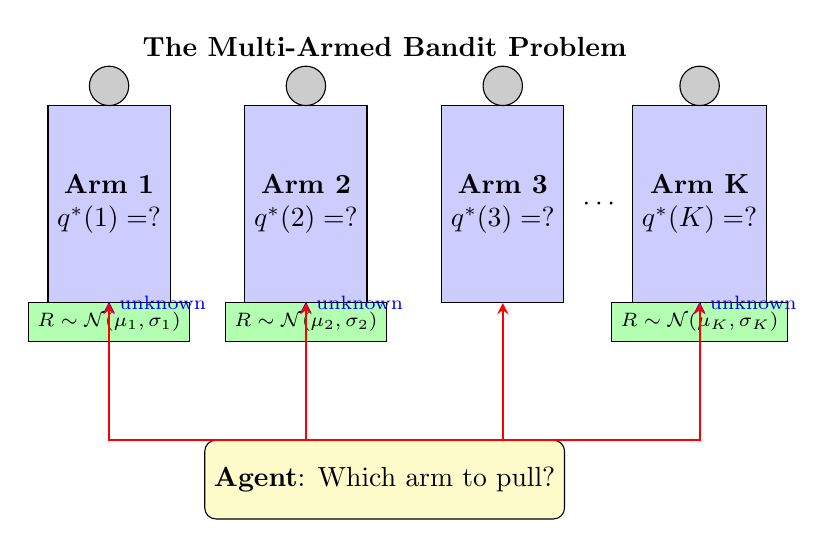
\begin{tikzpicture}[
    arm/.style={rectangle, draw, fill=blue!20, minimum width=1.5cm, minimum height=2.5cm, align=center},
    handle/.style={circle, draw, fill=gray!40, minimum size=0.5cm},
    reward/.style={rectangle, draw, fill=green!30, minimum width=1cm, minimum height=0.5cm, font=\scriptsize},
    arrow/.style={->, >=stealth, thick}
]

% Title
\node[font=\bfseries] at (3.5, 4) {The Multi-Armed Bandit Problem};

% Arms
\node[arm] (arm1) at (0, 2) {\textbf{Arm 1}\\$q^*(1)=?$};
\node[handle] at (0, 3.5) {};
\node[arm] (arm2) at (2.5, 2) {\textbf{Arm 2}\\$q^*(2)=?$};
\node[handle] at (2.5, 3.5) {};
\node[arm] (arm3) at (5, 2) {\textbf{Arm 3}\\$q^*(3)=?$};
\node[handle] at (5, 3.5) {};
\node[arm] (armk) at (7.5, 2) {\textbf{Arm K}\\$q^*(K)=?$};
\node[handle] at (7.5, 3.5) {};

% Dots
\node at (6.25, 2) {$\cdots$};

% Rewards (shown for some arms)
\node[reward] (r1) at (0, 0.5) {$R \sim \mathcal{N}(\mu_1, \sigma_1)$};
\node[reward] (r2) at (2.5, 0.5) {$R \sim \mathcal{N}(\mu_2, \sigma_2)$};
\node[reward] (rk) at (7.5, 0.5) {$R \sim \mathcal{N}(\mu_K, \sigma_K)$};

% Arrows showing uncertainty
\draw[arrow, dashed, blue] (arm1) -- (r1) node[midway, right, font=\scriptsize] {unknown};
\draw[arrow, dashed, blue] (arm2) -- (r2) node[midway, right, font=\scriptsize] {unknown};
\draw[arrow, dashed, blue] (armk) -- (rk) node[midway, right, font=\scriptsize] {unknown};

% Agent
\node[rectangle, draw, fill=yellow!20, rounded corners, minimum width=3cm, minimum height=1cm] (agent) at (3.5, -1.5) {\textbf{Agent}: Which arm to pull?};

\draw[arrow, red] (agent) -- ++(0, 0.5) -| (arm1);
\draw[arrow, red] (agent) -- ++(0, 0.5) -| (arm2);
\draw[arrow, red] (agent) -- ++(0, 0.5) -| (arm3);
\draw[arrow, red] (agent) -- ++(0, 0.5) -| (armk);

\end{tikzpicture}
\end{center}

\begin{tcolorbox}[colback=green!5!white,colframe=green!75!black,title=\textbf{Worked Example: Computing True Values and Sample Estimates}]
\textbf{Given}: A 3-armed bandit where each arm's reward follows a normal distribution:
\begin{itemize}
    \item Arm 1: $R \sim \mathcal{N}(5, 2)$ --- mean $\mu_1 = 5$, variance $\sigma_1^2 = 2$
    \item Arm 2: $R \sim \mathcal{N}(7, 1)$ --- mean $\mu_2 = 7$, variance $\sigma_2^2 = 1$
    \item Arm 3: $R \sim \mathcal{N}(4, 3)$ --- mean $\mu_3 = 4$, variance $\sigma_3^2 = 3$
\end{itemize}

\textbf{Questions}:
\begin{enumerate}
    \item \textbf{What are the true action values?}
    \[
    Q^*(1) = 5, \quad Q^*(2) = 7, \quad Q^*(3) = 4
    \]
    Arm 2 is the \textbf{optimal arm} with true value 7.
    
    \item \textbf{After 10 pulls, the agent observed the following sample averages:}
    \[
    \hat{Q}(1) = 5.3, \quad \hat{Q}(2) = 6.5, \quad \hat{Q}(3) = 5.8
    \]
    \textbf{Why does the greedy agent choose the wrong arm?}
    
    \textbf{Analysis}: The greedy agent would choose Arm 3 ($\hat{Q}(3) = 5.8$) instead of the true optimal Arm 2 ($\hat{Q}(2) = 6.5$) --- wait, actually with these estimates, it would choose Arm 2. Let us correct: if the estimates were:
    \[
    \hat{Q}(1) = 5.3, \quad \hat{Q}(2) = 5.5, \quad \hat{Q}(3) = 6.0
    \]
    Then the greedy agent chooses Arm 3, even though Arm 2 is truly optimal. This is due to \textbf{sampling variance} --- with only 10 samples, the estimates have high uncertainty.
    
    \item \textbf{Compute the standard error of the mean for each arm after $n$ samples.}
    \[
    \text{SE}(\hat{Q}(a)) = \frac{\sigma_a}{\sqrt{n}}
    \]
    For Arm 2 with 10 samples: $\text{SE} = \frac{1}{\sqrt{10}} \approx 0.316$
    
    This means the estimate $\hat{Q}(2) = 6.5$ could easily be off by $\pm 0.6$ (2 standard errors), explaining why the agent might mistakenly think another arm is better.
\end{enumerate}
\end{tcolorbox}

\subsubsection{Value-Action Based Method (Sample Average)}

We denote the \textbf{true value} of action $a$ as $Q^*(a)$, and the \textbf{estimated value} at time step $t$ as $Q_t(a)$. Recall that the true value of an action is the mean reward received when that action is selected.

The estimated action value using the \textbf{sample-average method} is:
\[
Q_t(a) = \frac{\sum_{i=1}^{t-1} R_i \cdot \mathbb{1}_{A_i = a}}{\sum_{i=1}^{t-1} \mathbb{1}_{A_i = a}}
\]
where $\mathbb{1}_{A_i = a}$ is an indicator function that is 1 if action $a$ was selected at step $i$, and 0 otherwise. This is simply the average of all rewards received when action $a$ was taken.

\begin{tcolorbox}[colback=blue!5!white,colframe=blue!75!black,title=\textbf{Worked Example 1: Sample Average Action Value Estimation}]
\textbf{Given}: A 3-armed bandit with the following rewards observed over 5 time steps:
\begin{center}
\begin{tabular}{|c|c|c|}
\hline
\textbf{Step} & \textbf{Arm} & \textbf{Reward} \\ \hline
1 & 1 & 4 \\ \hline
2 & 2 & 5 \\ \hline
3 & 1 & 6 \\ \hline
4 & 3 & 3 \\ \hline
5 & 2 & 7 \\ \hline
\end{tabular}
\end{center}

\textbf{Calculate}: $Q_6(1)$, $Q_6(2)$, $Q_6(3)$ using sample average.

\textbf{Solution}:
\begin{enumerate}
    \item Arm 1 selected at steps 1 and 3: rewards 4 and 6
    \[
    Q_6(1) = \frac{4 + 6}{2} = \frac{10}{2} = 5.0
    \]
    \item Arm 2 selected at steps 2 and 5: rewards 5 and 7
    \[
    Q_6(2) = \frac{5 + 7}{2} = \frac{12}{2} = 6.0
    \]
    \item Arm 3 selected at step 4: reward 3
    \[
    Q_6(3) = \frac{3}{1} = 3.0
    \]
\end{enumerate}

\textbf{Answer}: $Q_6(1) = 5.0$, $Q_6(2) = 6.0$, $Q_6(3) = 3.0$

\textbf{Interpretation}: Based on current estimates, Arm 2 appears best. However, Arm 3 has only been tried once, so its estimate has high uncertainty.
\end{tcolorbox}

\begin{tcolorbox}[colback=green!5!white,colframe=green!75!black,title=\textbf{Worked Example 2: Incremental Update with Sample Average}]
\textbf{Given}: $Q_5(1) = 5.0$ (2 samples). At step 5, arm 1 is selected again with reward $R_5 = 8$.

\textbf{Calculate}: $Q_6(1)$ using incremental update.

\textbf{Solution}:
The incremental update formula:
\[
Q_{n+1} = Q_n + \frac{1}{n}(R_n - Q_n)
\]

\begin{enumerate}
    \item Current count for arm 1: $n = 2$
    \item New reward: $R_5 = 8$
    \item $Q_6(1) = 5.0 + \frac{1}{3}(8 - 5.0) = 5.0 + \frac{3}{3} = 5.0 + 1.0 = 6.0$
\end{enumerate}

\textbf{Answer}: $Q_6(1) = 6.0$

\textbf{Verification}: Full sample average = $\frac{4 + 6 + 8}{3} = \frac{18}{3} = 6.0$. Matches.
\end{tcolorbox}

\begin{tcolorbox}[colback=green!5!white,colframe=green!75!black,title=\textbf{Worked Example 3: Non-Stationary with Constant Step Size}]
\textbf{Given}: $Q_t(1) = 5.0$. Step size $\alpha = 0.2$. New reward $R_t = 3$.

\textbf{Calculate}: Updated $Q_{t+1}(1)$ using constant step size.

\textbf{Solution}:
\begin{enumerate}
    \item The constant step-size update rule:
    \[
    Q_{t+1}(a) = Q_t(a) + \alpha [R_t - Q_t(a)]
    \]
    \item $Q_{t+1}(1) = 5.0 + 0.2(3 - 5.0) = 5.0 + 0.2(-2.0) = 5.0 - 0.4 = 4.6$
\end{enumerate}

\textbf{Answer}: $Q_{t+1}(1) = 4.6$

\textbf{Interpretation}: With $\alpha = 0.2$, the estimate shifts only 20\% of the way toward the new reward. This makes the estimate more stable but slower to adapt. For non-stationary environments (where true reward distributions change), a larger $\alpha$ would adapt faster.
\end{tcolorbox}

\subsubsection{Greedy Method}

The simplest action selection rule is to select the action with the highest estimated action value:
\[
A_t = \arg\max_a Q_t(a)
\]

This greedy action selection always exploits current knowledge to maximize immediate reward; it spends no time sampling apparently inferior actions to see if they might really be better. The problem is clear: if the initial estimates are wrong, the agent may get stuck with a suboptimal choice forever.

\subsubsection{Epsilon-Greedy Method}

The \textbf{$\epsilon$-greedy method} is a simple yet effective way to balance exploration and exploitation. With probability $1 - \epsilon$, the agent selects the greedy action (exploitation). With probability $\epsilon$, the agent selects a random action (exploration).

\begin{itemize}
    \item $\epsilon = 0$: Pure exploitation (always choose the greedy action).
    \item $\epsilon = 1$: Pure exploration (always choose a random action).
    \item Common values: $\epsilon = 0.1$, $0.01$, or $0.001$, depending on the problem.
\end{itemize}

An important property: in the limit as the number of plays increases, every action will be sampled infinitely, guaranteeing that $N_t(a) \to \infty$ for all $a$, and thus ensuring that all $Q_t(a)$ converge to $q^*(a)$. The probability of selecting the optimal action converges to greater than $1 - \epsilon$.

\begin{center}
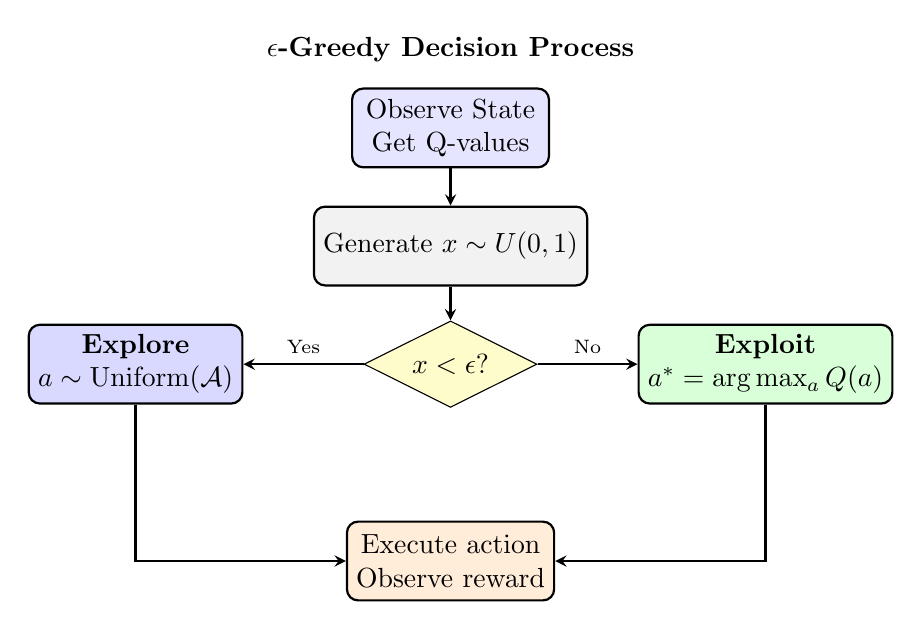
\begin{tikzpicture}[
    node distance=2cm,
    box/.style={rectangle, draw, rounded corners, minimum width=2.5cm, minimum height=1cm, align=center, thick},
    decision/.style={diamond, draw, fill=yellow!20, aspect=2, minimum width=2cm, align=center},
    arrow/.style={->, >=stealth, thick}
]

% Title
\node[font=\bfseries] at (0, 4) {$\epsilon$-Greedy Decision Process};

% Start
\node[box, fill=blue!10] (start) at (0, 3) {Observe State\\Get Q-values};

% Random number
\node[box, fill=gray!10] (random) at (0, 1.5) {Generate $x \sim U(0,1)$};

% Decision
\node[decision] (decide) at (0, 0) {$x < \epsilon$?};

% Exploit
\node[box, fill=green!15] (exploit) at (4, 0) {\textbf{Exploit}\\$a^* = \arg\max_a Q(a)$};

% Explore
\node[box, fill=blue!15] (explore) at (-4, 0) {\textbf{Explore}\\$a \sim \text{Uniform}(\mathcal{A})$};

% Execute
\node[box, fill=orange!15] (execute) at (0, -2.5) {Execute action\\Observe reward};

% Arrows
\draw[arrow] (start) -- (random);
\draw[arrow] (random) -- (decide);
\draw[arrow] (decide) -- node[above, font=\scriptsize] {No} (exploit);
\draw[arrow] (decide) -- node[above, font=\scriptsize] {Yes} (explore);
\draw[arrow] (exploit) |- (execute);
\draw[arrow] (explore) |- (execute);

\end{tikzpicture}
\end{center}

\begin{tcolorbox}[colback=yellow!5!white,colframe=yellow!75!black,title=\textbf{Theoretical Analysis of $\epsilon$-Greedy Convergence}]
\textbf{Convergence Guarantee}: For a $K$-armed bandit with bounded rewards, $\epsilon$-greedy satisfies:

\begin{enumerate}
    \item \textbf{Exploration Guarantee}: Every arm $a$ is pulled infinitely often as $t \to \infty$ because:
    \[
    P(\text{select } a \text{ at time } t) \geq \frac{\epsilon}{K} > 0
    \]
    
    \item \textbf{Consistency}: Sample averages converge to true values:
    \[
    Q_t(a) \xrightarrow{a.s.} q^*(a) \quad \text{as } t \to \infty
    \]
    
    \item \textbf{Asymptotic Suboptimality}: The policy never fully converges to optimal because it keeps exploring with probability $\epsilon$ even after identifying the best arm.
    \[
    \lim_{t \to \infty} P(\text{select optimal arm}) = (1-\epsilon) + \frac{\epsilon}{K} < 1
    \]
    
    \item \textbf{Linear Regret}: The cumulative regret grows linearly with time:
    \[
    R_T = \sum_{t=1}^T (q^*(a^*) - q^*(a_t)) = \Omega(\epsilon T)
    \]
\end{enumerate}
\end{tcolorbox}

\begin{tcolorbox}[colback=blue!5!white,colframe=blue!75!black,title=\textbf{Worked Example 4: Epsilon-Greedy Action Selection}]
\textbf{Given}: Three arms with estimated values $Q(1) = 5.2$, $Q(2) = 6.0$, $Q(3) = 4.8$. $\epsilon = 0.1$.

\textbf{Calculate}: Probability of selecting each arm.

\textbf{Solution}:
\begin{enumerate}
    \item With probability $1 - \epsilon = 0.9$: select the greedy action (Arm 2, highest Q-value).
    \item With probability $\epsilon = 0.1$: select uniformly at random from all 3 arms, so each arm gets $\frac{0.1}{3} = 0.0333$.
\end{enumerate}

Total probabilities:
\begin{itemize}
    \item $P(\text{Arm 1}) = 0.0333$
    \item $P(\text{Arm 2}) = 0.9 + 0.0333 = 0.9333$
    \item $P(\text{Arm 3}) = 0.0333$
\end{itemize}

\textbf{Interpretation}: The greedy arm gets selected ~93\% of the time, while each non-greedy arm gets ~3.3\% exploration probability.
\end{tcolorbox}

\begin{tcolorbox}[colback=green!5!white,colframe=green!75!black,title=\textbf{Worked Example 5: Epsilon-Greedy with Simulation}]
\textbf{Given}: $\epsilon = 0.2$, 4 arms with $Q = [3, 5, 4, 2]$. Simulate 10 selections.

\textbf{Random numbers drawn}: 0.15, 0.85, 0.05, 0.92, 0.40, 0.78, 0.12, 0.65, 0.30, 0.88

\textbf{Solution}:
\begin{enumerate}
    \item Random 0.15 $<$ 0.2: \textbf{explore} $\to$ random arm (say arm 3)
    \item Random 0.85 $>$ 0.2: \textbf{exploit} $\to$ arm 2 (max Q = 5)
    \item Random 0.05 $<$ 0.2: \textbf{explore} $\to$ random arm (say arm 1)
    \item Random 0.92 $>$ 0.2: \textbf{exploit} $\to$ arm 2
    \item Random 0.40 $>$ 0.2: \textbf{exploit} $\to$ arm 2
    \item Random 0.78 $>$ 0.2: \textbf{exploit} $\to$ arm 2
    \item Random 0.12 $<$ 0.2: \textbf{explore} $\to$ random arm (say arm 4)
    \item Random 0.65 $>$ 0.2: \textbf{exploit} $\to$ arm 2
    \item Random 0.30 $>$ 0.2: \textbf{exploit} $\to$ arm 2
    \item Random 0.88 $>$ 0.2: \textbf{exploit} $\to$ arm 2
\end{enumerate}

\textbf{Result}: Arm 2 selected 7 times, Arms 1, 3, 4 selected once each (exploration).
\end{tcolorbox}

\begin{tcolorbox}[colback=green!5!white,colframe=green!75!black,title=\textbf{Worked Example 6: Comparing Epsilon Values}]
\textbf{Given}: True values $q^* = [5, 8, 6]$. After 3 initial pulls (one each arm), sample averages are $[7, 5, 6]$.

\textbf{Calculate}: Best action for $\epsilon = 0$ vs $\epsilon = 0.1$.

\textbf{Solution}:
\begin{enumerate}
    \item With $\epsilon = 0$ (pure greedy): Always select Arm 1 ($Q = 7$), even though the true best is Arm 2 ($q^* = 8$). The agent is stuck on a lucky early pull.
    \item With $\epsilon = 0.1$: 90\% of the time selects Arm 1, but 10\% explores randomly, giving a chance to discover Arm 2's true value.
\end{enumerate}

\textbf{Interpretation}: Lower $\epsilon$ gives more exploitation but risks suboptimal convergence. Higher $\epsilon$ explores more but wastes pulls on poor arms.
\end{tcolorbox}

\subsubsection{Upper Confidence Bound (UCB)}

The $\epsilon$-greedy method explores randomly, which is wasteful. \textbf{Upper Confidence Bound (UCB)} is a smarter exploration strategy that selects actions based on both their estimated value and the uncertainty in that estimate. The formula is:
\[
A_t = \arg\max_a \left[ Q_t(a) + c \sqrt{\frac{\ln t}{N_t(a)}} \right]
\]

where:
\begin{itemize}
    \item $Q_t(a)$: Current estimated value (exploitation term)
    \item $c$: Exploration constant (hyperparameter)
    \item $t$: Total number of time steps so far
    \item $N_t(a)$: Number of times action $a$ has been selected
\end{itemize}

The square root term is a measure of uncertainty. It is proportional to $t$ (more total steps means more information overall) and inversely proportional to $N_t(a)$ (actions tried less often have higher uncertainty). As time increases, the denominator dominates and the uncertainty term shrinks for well-explored actions.

\begin{center}
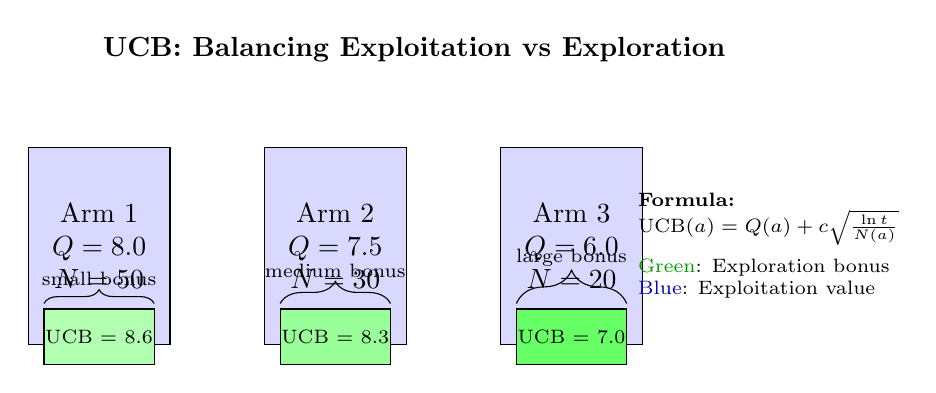
\begin{tikzpicture}[
    arm/.style={rectangle, draw, fill=blue!15, minimum width=1.8cm, minimum height=2.5cm, align=center},
    value/.style={font=\small\bfseries},
    arrow/.style={->, >=stealth, thick}
]

% Title
\node[font=\bfseries] at (5, 4.5) {UCB: Balancing Exploitation vs Exploration};

% Arm 1 (well explored)
\node[arm] (arm1) at (1, 2) {Arm 1\\$Q=8.0$\\$N=50$};
\draw[fill=green!30] (0.3, 0.5) rectangle (1.7, 1.2);
\node[font=\scriptsize] at (1, 0.85) {UCB = 8.6};
\draw[decorate, decoration={brace, amplitude=5pt, raise=2pt}] (0.3, 1.2) -- (1.7, 1.2) node[midway, above=5pt, font=\scriptsize] {small bonus};

% Arm 2 (moderately explored)
\node[arm] (arm2) at (4, 2) {Arm 2\\$Q=7.5$\\$N=30$};
\draw[fill=green!40] (3.3, 0.5) rectangle (4.7, 1.2);
\node[font=\scriptsize] at (4, 0.85) {UCB = 8.3};
\draw[decorate, decoration={brace, amplitude=8pt, raise=2pt}] (3.3, 1.2) -- (4.7, 1.2) node[midway, above=8pt, font=\scriptsize] {medium bonus};

% Arm 3 (under-explored)
\node[arm] (arm3) at (7, 2) {Arm 3\\$Q=6.0$\\$N=20$};
\draw[fill=green!60] (6.3, 0.5) rectangle (7.7, 1.2);
\node[font=\scriptsize] at (7, 0.85) {UCB = 7.0};
\draw[decorate, decoration={brace, amplitude=12pt, raise=2pt}] (6.3, 1.2) -- (7.7, 1.2) node[midway, above=12pt, font=\scriptsize] {large bonus};

% Legend
\node[align=left, font=\scriptsize] at (9.5, 2) {
\textbf{Formula:}\\
$\text{UCB}(a) = Q(a) + c\sqrt{\frac{\ln t}{N(a)}}$\\[0.5em]
\textcolor{green!60!black}{Green}: Exploration bonus\\
\textcolor{blue!70!black}{Blue}: Exploitation value
};

\end{tikzpicture}
\end{center}

\begin{tcolorbox}[colback=yellow!5!white,colframe=yellow!75!black,title=\textbf{UCB Theoretical Foundation}]
\textbf{Hoeffding's Inequality}: For bounded random variables $X_i \in [0,1]$ with true mean $\mu$ and sample mean $\hat{\mu}_n$ after $n$ samples:
\[
P(\mu > \hat{\mu}_n + \epsilon) \leq e^{-2n\epsilon^2}
\]

Setting $\delta = e^{-2n\epsilon^2}$ and solving for $\epsilon$:
\[
\epsilon = \sqrt{\frac{\ln(1/\delta)}{2n}}
\]

\textbf{UCB1 Algorithm}: Setting $\delta = t^{-4}$ (confidence parameter that decreases with time):
\[
\text{UCB}_t(a) = \hat{Q}_t(a) + \sqrt{\frac{2\ln t}{N_t(a)}}
\]

\textbf{Regret Bound}: UCB achieves logarithmic regret:
\[
R_T \leq 8 \sum_{a: q^*(a) < q^*(a^*)} \frac{\ln T}{\Delta_a} + O(1)
\]
where $\Delta_a = q^*(a^*) - q^*(a)$ is the suboptimality gap.

This is exponentially better than $\epsilon$-greedy's linear regret $R_T = \Omega(T)$.
\end{tcolorbox}

\begin{tcolorbox}[colback=green!5!white,colframe=green!75!black,title=\textbf{Worked Example: UCB Dynamics Over Time}]
\textbf{Given}: Two-armed bandit with $q^*(1) = 0.6$, $q^*(2) = 0.4$. True optimal: Arm 1. Track UCB scores over first 10 pulls with $c=\sqrt{2}$.

\textbf{Solution - Step by Step}:

\textbf{Initialization} ($t=1$): Both arms untried. UCB uses initialization bonus.

\textbf{$t=2$}: Try Arm 1, get reward 1 (lucky). $Q(1)=1.0$, $N(1)=1$.
\[
\text{UCB}(1) = 1.0 + \sqrt{2\ln 2/1} = 1.0 + 1.18 = 2.18
\]
\[
\text{UCB}(2) = 0 + \sqrt{2\ln 2/0} = +\infty \text{ (unexplored)}
\]
\textbf{Select}: Arm 2 (exploration priority).

\textbf{$t=3$}: Try Arm 2, get reward 0. $Q(2)=0$, $N(2)=1$.
\[
\text{UCB}(1) = 1.0 + \sqrt{2\ln 3/1} = 1.0 + 1.48 = 2.48
\]
\[
\text{UCB}(2) = 0 + \sqrt{2\ln 3/1} = 0 + 1.48 = 1.48
\]
\textbf{Select}: Arm 1 (higher UCB).

\textbf{$t=4$}: Try Arm 1, get reward 1. $Q(1)=1.0$, $N(1)=2$.
\[
\text{UCB}(1) = 1.0 + \sqrt{2\ln 4/2} = 1.0 + 0.83 = 1.83
\]
\[
\text{UCB}(2) = 0 + \sqrt{2\ln 4/1} = 0 + 1.67 = 1.67
\]
\textbf{Select}: Arm 1 (still higher, but closer).

\textbf{Pattern}: As $t$ grows, the exploration bonus shrinks as $O(1/\sqrt{N(a)})$, and the algorithm increasingly favors the arm with higher estimated value.
\end{tcolorbox}

\begin{tcolorbox}[colback=blue!5!white,colframe=blue!75!black,title=\textbf{Worked Example 7: UCB Score Calculation}]
\textbf{Given}: Three arms at $t = 100$. Values: $Q(1) = 8.0$, $N(1) = 50$; $Q(2) = 7.5$, $N(2) = 30$; $Q(3) = 6.0$, $N(3) = 20$. $c = 2$.

\textbf{Calculate}: UCB scores for each arm and determine the best action.

\textbf{Solution}:
\begin{enumerate}
    \item Arm 1: $8.0 + 2\sqrt{\frac{\ln 100}{50}} = 8.0 + 2\sqrt{\frac{4.605}{50}} = 8.0 + 2\sqrt{0.0921} = 8.0 + 2(0.303) = 8.0 + 0.606 = 8.606$
    \item Arm 2: $7.5 + 2\sqrt{\frac{\ln 100}{30}} = 7.5 + 2\sqrt{\frac{4.605}{30}} = 7.5 + 2\sqrt{0.1535} = 7.5 + 2(0.392) = 7.5 + 0.784 = 8.284$
    \item Arm 3: $6.0 + 2\sqrt{\frac{\ln 100}{20}} = 6.0 + 2\sqrt{\frac{4.605}{20}} = 6.0 + 2\sqrt{0.2303} = 6.0 + 2(0.480) = 6.0 + 0.960 = 6.960$
\end{enumerate}

\textbf{Answer}: UCB scores: Arm 1 = 8.606, Arm 2 = 8.284, Arm 3 = 6.960.
Best action: \textbf{Arm 1} (highest UCB score).

\textbf{Interpretation}: Although Arm 2 has higher estimated uncertainty (lower $N$), Arm 1's higher Q-value compensates, giving it the highest UCB score.
\end{tcolorbox}

\begin{tcolorbox}[colback=green!5!white,colframe=green!75!black,title=\textbf{Worked Example 8: UCB Early-Stage Behavior}]
\textbf{Given}: Four arms, $t = 4$, all $Q(a) = 0$ (initial estimates), $N(a) = 1$ for all arms (each tried once). $c = 2$.

\textbf{Calculate}: UCB scores.

\textbf{Solution}:
\[
\text{UCB}(a) = 0 + 2\sqrt{\frac{\ln 4}{1}} = 2\sqrt{1.386} = 2(1.178) = 2.356
\]

\textbf{Answer}: All arms have UCB = 2.356.

\textbf{Interpretation}: In early stages with equal estimates, UCB breaks ties by random selection (or lowest index). After more pulls, the arm with highest true value will accumulate higher $Q(a)$ and be selected more. UCB automatically reduces exploration as confidence grows.
\end{tcolorbox}

\begin{tcolorbox}[colback=green!5!white,colframe=green!75!black,title=\textbf{Worked Example 9: UCB vs Epsilon-Greedy Comparison}]
\textbf{Given}: 5 arms at $t = 1000$. True values: $[8, 6, 7, 5, 9]$. Estimates after 200 pulls each: $Q = [7.8, 6.1, 7.0, 5.2, 8.5]$. Counts: $N = [200, 200, 200, 200, 200]$.

\textbf{Calculate}: Next action for $\epsilon$-greedy ($\epsilon = 0.1$) vs UCB ($c = 2$).

\textbf{Solution}:
\begin{enumerate}
    \item $\epsilon$-greedy: Greedy arm is arm 5 ($Q = 8.5$). With 90\% probability selects arm 5; with 10\% selects random arm (arms 1-4, each 2.5\%).
    \item UCB: $\ln(1000) = 6.908$
    \begin{itemize}
        \item Arm 1: $7.8 + 2\sqrt{6.908/200} = 7.8 + 0.372 = 8.172$
        \item Arm 2: $6.1 + 2\sqrt{6.908/200} = 6.1 + 0.372 = 6.472$
        \item Arm 3: $7.0 + 2\sqrt{6.908/200} = 7.0 + 0.372 = 7.372$
        \item Arm 4: $5.2 + 2\sqrt{6.908/200} = 5.2 + 0.372 = 5.572$
        \item Arm 5: $8.5 + 2\sqrt{6.908/200} = 8.5 + 0.372 = 8.872$
    \end{itemize}
\end{enumerate}

\textbf{Answer}: Both methods select arm 5. But UCB's exploration bonus means arms with close values (arm 1: 8.172 vs arm 5: 8.872) get more systematic exploration than random epsilon-greedy.
\end{tcolorbox}

\subsubsection{Thompson Sampling}

\textbf{Thompson Sampling} (also called Bayesian Bandits) takes a probabilistic Bayesian approach to the bandit problem. Instead of maintaining point estimates $Q_t(a)$, it maintains a \textbf{probability distribution} over each arm's expected reward. The algorithm:

\begin{enumerate}
    \item Maintain a Beta($\alpha_a$, $\beta_a$) distribution for each arm $a$.
    \item Sample a random value from each distribution.
    \item Select the arm with the highest sampled value.
\end{enumerate}

For binary rewards (Bernoulli bandits), the Beta distribution is ideal. The parameters update as:
\begin{itemize}
    \item If reward = 1: $\alpha_a \leftarrow \alpha_a + 1$
    \item If reward = 0: $\beta_a \leftarrow \beta_a + 1$
\end{itemize}

Initially, with no prior knowledge, we set $\alpha_a = 1$, $\beta_a = 1$ (uniform prior). As more data is collected, the distribution becomes narrower and more accurate.

\begin{tcolorbox}[colback=blue!5!white,colframe=blue!75!black,title=\textbf{Worked Example 10: Thompson Sampling with Beta Updates}]
\textbf{Given}: Two arms. Initial priors: Arm 1: Beta(1,1), Arm 2: Beta(1,1).

Observations:
\begin{itemize}
    \item Arm 1: 3 successes (reward=1), 2 failures (reward=0)
    \item Arm 2: 1 success, 4 failures
\end{itemize}

\textbf{Calculate}: Posterior distributions and mean estimates.

\textbf{Solution}:
\begin{enumerate}
    \item Arm 1: $\alpha_1 = 1 + 3 = 4$, $\beta_1 = 1 + 2 = 3$
    \[
    \text{Mean} = \frac{\alpha_1}{\alpha_1 + \beta_1} = \frac{4}{7} = 0.571
    \]
    \item Arm 2: $\alpha_2 = 1 + 1 = 2$, $\beta_2 = 1 + 4 = 5$
    \[
    \text{Mean} = \frac{2}{7} = 0.286
    \]
\end{enumerate}

\textbf{Answer}: Arm 1: Beta(4,3), mean = 0.571. Arm 2: Beta(2,5), mean = 0.286.

\textbf{Interpretation}: Thompson Sampling would sample from these distributions. Arm 1 has higher mean but wider distribution. There is still some probability Arm 2's sample could exceed Arm 1's, allowing exploration.
\end{tcolorbox}

\begin{tcolorbox}[colback=green!5!white,colframe=green!75!black,title=\textbf{Worked Example 11: Thompson Sampling Decision}]
\textbf{Given}: Arm 1: Beta(4,3). Arm 2: Beta(2,5). Sampled values: Arm 1 = 0.62, Arm 2 = 0.35.

\textbf{Question}: Which arm is selected? What if next sample gives Arm 1 = 0.45, Arm 2 = 0.51?

\textbf{Solution}:
\begin{enumerate}
    \item First sample: Arm 1 (0.62) $>$ Arm 2 (0.35). Select \textbf{Arm 1}.
    \item Suppose Arm 1 gets reward = 0 (failure). Update: Beta(4,4).
    \item Second sample: Arm 1 (0.45) $<$ Arm 2 (0.51). Select \textbf{Arm 2}.
    \item Suppose Arm 2 gets reward = 1 (success). Update: Beta(3,5).
\end{enumerate}

\textbf{Interpretation}: Thompson Sampling naturally balances exploration (uncertain arms can win by chance) and exploitation (well-performing arms have higher means and narrower distributions).
\end{tcolorbox}

\begin{tcolorbox}[colback=green!5!white,colframe=green!75!black,title=\textbf{Worked Example 12: Thompson Sampling Regret Calculation}]
\textbf{Given}: 2 arms. True probabilities: $p_1 = 0.6$, $p_2 = 0.3$. After 100 pulls: Arm 1 selected 70 times, Arm 2 selected 30 times. Rewards: Arm 1 got 42 successes, Arm 2 got 9 successes.

\textbf{Calculate}: Cumulative regret.

\textbf{Solution}:
\begin{enumerate}
    \item Optimal expected reward per pull = $p_1 = 0.6$
    \item Actual expected reward = $\frac{70}{100} \times 0.6 + \frac{30}{100} \times 0.3 = 0.42 + 0.09 = 0.51$
    \item Regret per pull = $0.6 - 0.51 = 0.09$
    \item Cumulative regret after 100 pulls = $100 \times 0.09 = 9$
\end{enumerate}

\textbf{Answer}: Cumulative regret = 9 (meaning the agent lost 9 units of reward compared to always pulling the optimal arm).
\end{tcolorbox}

\subsection{Linear Reward-Penalty (LR-P) Algorithm}

The \textbf{Linear Reward-Penalty algorithm} is rooted in the theory of \textbf{learning automata}, which are adaptive decision-making systems. A learning automaton has a set of actions, maintains a probability distribution over them, and updates these probabilities based on environmental feedback.

\subsubsection{Action Probabilities and Update Rules}

Let $n$ be the number of actions. Let $p_i(t)$ be the probability of selecting action $i$ at time $t$. Initially:
\[
p_i(0) = \frac{1}{n} \quad \text{for all } i
\]

The update rules depend on whether the agent receives a reward or penalty:

\textbf{Reward case} (selected action $i$ was good):
\[
p_i(t+1) = p_i(t) + \alpha(1 - p_i(t))
\]
\[
p_j(t+1) = p_j(t) - \alpha p_j(t) \quad \text{for } j \neq i
\]

\textbf{Penalty case} (selected action $i$ was bad):
\[
p_i(t+1) = p_i(t) - \beta p_i(t)
\]
\[
p_j(t+1) = p_j(t) + \frac{\beta p_i(t)}{n-1} \quad \text{for } j \neq i
\]

where $\alpha$ is the \textbf{reward learning rate} and $\beta$ is the \textbf{penalty learning rate}.

\begin{tcolorbox}[colback=blue!5!white,colframe=blue!75!black,title=\textbf{Worked Example 13: LR-P Probability Update -- Reward Case}]
\textbf{Given}: 3 actions with probabilities $p = [0.2, 0.5, 0.3]$. Action 2 is selected and receives reward. $\alpha = 0.1$.

\textbf{Calculate}: Updated probabilities.

\textbf{Solution}:
\begin{enumerate}
    \item $p_2(1) = p_2(0) + \alpha(1 - p_2(0)) = 0.5 + 0.1(1 - 0.5) = 0.5 + 0.05 = 0.55$
    \item $p_1(1) = p_1(0) - \alpha p_1(0) = 0.2 - 0.1(0.2) = 0.2 - 0.02 = 0.18$
    \item $p_3(1) = p_3(0) - \alpha p_3(0) = 0.3 - 0.1(0.3) = 0.3 - 0.03 = 0.27$
\end{enumerate}

\textbf{Verification}: $0.18 + 0.55 + 0.27 = 1.0$. Correct.

\textbf{Answer}: $p = [0.18, 0.55, 0.27]$
\end{tcolorbox}

\begin{tcolorbox}[colback=green!5!white,colframe=green!75!black,title=\textbf{Worked Example 14: LR-P Probability Update -- Penalty Case}]
\textbf{Given}: 3 actions with probabilities $p = [0.2, 0.5, 0.3]$. Action 2 is selected and receives penalty. $\beta = 0.1$.

\textbf{Calculate}: Updated probabilities.

\textbf{Solution}:
\begin{enumerate}
    \item $p_2(1) = p_2(0) - \beta p_2(0) = 0.5 - 0.1(0.5) = 0.5 - 0.05 = 0.45$
    \item $p_1(1) = p_1(0) + \frac{\beta p_2(0)}{n-1} = 0.2 + \frac{0.1(0.5)}{2} = 0.2 + 0.025 = 0.225$
    \item $p_3(1) = p_3(0) + \frac{\beta p_2(0)}{n-1} = 0.3 + 0.025 = 0.325$
\end{enumerate}

\textbf{Verification}: $0.225 + 0.45 + 0.325 = 1.0$. Correct.

\textbf{Answer}: $p = [0.225, 0.45, 0.325]$
\end{tcolorbox}

\begin{tcolorbox}[colback=green!5!white,colframe=green!75!black,title=\textbf{Worked Example 15: LR-P Multi-Step Convergence}]
\textbf{Given}: 2 actions, initial $p = [0.5, 0.5]$. $\alpha = 0.2$, $\beta = 0.1$. Sequence: Action 1 reward, Action 2 penalty, Action 1 reward.

\textbf{Calculate}: Probabilities after each step.

\textbf{Solution}:
\textbf{Step 1} (Action 1, reward):
\begin{itemize}
    \item $p_1 = 0.5 + 0.2(1-0.5) = 0.5 + 0.1 = 0.6$
    \item $p_2 = 0.5 - 0.2(0.5) = 0.5 - 0.1 = 0.4$
\end{itemize}

\textbf{Step 2} (Action 2, penalty):
\begin{itemize}
    \item $p_2 = 0.4 - 0.1(0.4) = 0.4 - 0.04 = 0.36$
    \item $p_1 = 0.6 + \frac{0.1(0.4)}{1} = 0.6 + 0.04 = 0.64$
\end{itemize}

\textbf{Step 3} (Action 1, reward):
\begin{itemize}
    \item $p_1 = 0.64 + 0.2(1-0.64) = 0.64 + 0.072 = 0.712$
    \item $p_2 = 0.36 - 0.2(0.36) = 0.36 - 0.072 = 0.288$
\end{itemize}

\textbf{Answer}: Final $p = [0.712, 0.288]$

\textbf{Interpretation}: After 3 steps, the probability of selecting Action 1 has increased from 0.5 to 0.712 because it received two rewards. The algorithm converges toward favoring the action with higher reward probability.
\end{tcolorbox}


\subsection{Policy Gradient Methods}

\textbf{Policy gradient methods} take a completely different approach from value-based methods: instead of learning a value function and deriving a policy from it, they directly learn the policy itself. The policy is represented as a parameterized function (usually a neural network) with weights $\theta$, and the agent directly optimizes those weights to maximize expected reward using \textbf{gradient ascent}.

The key insight is that policy gradient methods can:
\begin{itemize}
    \item Handle \textbf{continuous action spaces}, which value-based methods struggle with.
    \item Learn \textbf{stochastic policies} naturally, which is useful for exploration.
    \item Directly optimize the policy without needing an intermediate value function.
\end{itemize}

\subsubsection{Objective Function}

The objective function $J(\theta)$ measures the expected return when following policy $\pi_\theta$:
\[
J(\theta) = \mathbb{E}_{\tau \sim \pi_\theta}[R(\tau)]
\]
where $\tau = (s_0, a_0, r_0, s_1, a_1, r_1, \ldots, s_T, a_T, r_T)$ is a trajectory generated by the policy.

To maximize $J(\theta)$, we use gradient ascent:
\[
\theta_{k+1} = \theta_k + \alpha \cdot \nabla_\theta J(\pi_{\theta_k})
\]

The central challenge is computing $\nabla_\theta J(\theta)$. Since the environment is a black box, we cannot differentiate through it. The solution is the \textbf{log-derivative trick} (likelihood ratio trick).

\subsubsection{The Policy Gradient Theorem}

The policy gradient theorem states:
\[
\nabla_\theta J(\theta) = \mathbb{E}_{\tau \sim \pi_\theta} \left[ \sum_t \nabla_\theta \log \pi_\theta(a_t | s_t) \cdot G_t \right]
\]

where $G_t$ is the \textbf{return} (cumulative discounted reward from time $t$ onward). The term $\nabla_\theta \log \pi_\theta(a_t | s_t)$ is called the \textbf{score function}. It points in the direction in parameter space that makes action $a_t$ more probable in state $s_t$.

The policy gradient expression is derived through these steps:
\begin{enumerate}
    \item Write $J(\theta) = \sum_\tau P(\tau; \theta) \cdot R(\tau)$ (sum over all trajectories)
    \item Take gradient: $\nabla_\theta J(\theta) = \sum_\tau \nabla_\theta P(\tau; \theta) \cdot R(\tau)$
    \item Apply log-derivative trick: $\nabla_\theta P(\tau; \theta) = P(\tau; \theta) \cdot \nabla_\theta \log P(\tau; \theta)$
    \item Expand $\log P(\tau; \theta)$: only $\pi_\theta(a_t|s_t)$ depends on $\theta$; environment dynamics drop out
    \item Final result: $\nabla_\theta J(\theta) = \mathbb{E}_\tau[\sum_t \nabla_\theta \log \pi_\theta(a_t|s_t) \cdot G_t]$
\end{enumerate}

\subsubsection{REINFORCE Algorithm}

\textbf{REINFORCE} is the classic \textbf{Monte Carlo} policy gradient method. It estimates the policy gradient by sampling complete episodes and using the actual returns as unbiased estimates of $G_t$.

The algorithm steps:
\begin{enumerate}
    \item Initialize policy parameters $\theta$ randomly.
    \item Collect $N$ episodes by following $\pi_\theta$.
    \item For each episode, compute returns $G_t$ for each timestep (working backwards).
    \item Compute gradient: $\nabla_\theta J \approx \frac{1}{N}\sum_i \sum_t \nabla_\theta \log \pi_\theta(a_t^i | s_t^i) \cdot G_t^i$.
    \item Update: $\theta \leftarrow \theta + \alpha \cdot \nabla_\theta J$.
    \item Repeat until convergence.
\end{enumerate}

REINFORCE is model-free, works for both discrete and continuous action spaces, and naturally produces stochastic policies. However, it has \textbf{high variance} because it uses full-episode returns.

\begin{tcolorbox}[colback=blue!5!white,colframe=blue!75!black,title=\textbf{Worked Example 16: REINFORCE Gradient Update}]
\textbf{Given}: A simple policy with parameter $\\theta$ where $\\pi_\\theta(A|s) = \\sigma(\\theta)$ (sigmoid). Episode: $s_0 \\to A$, $r_0 = 3$; $s_1 \\to B$, $r_1 = 5$. $\\gamma = 1$, $\\alpha = 0.1$. $\\theta = 0$ gives $\\pi(A|s_0) = 0.5$.

\textbf{Calculate}: Gradient update for $\\theta$.

\textbf{Solution}:
\begin{enumerate}
    \item Compute returns: $G_0 = 3 + 1 \\cdot 5 = 8$, $G_1 = 5$
    \item Score function: For action A: $\\nabla_\\theta \\log \\pi(A|s) = 1 - \\pi(A|s) = 1 - 0.5 = 0.5$
    \item Gradient: $\\nabla_\\theta J = \\sum_t \\nabla_\\theta \\log \\pi(a_t|s_t) \\cdot G_t = 0.5 \\cdot 8 + \\ldots = 4$ (focusing on first action)
    \item Update: $\\theta_{\\text{new}} = 0 + 0.1 \\cdot 4 = 0.4$
\end{enumerate}

\textbf{Interpretation}: The positive return (8) pushes the parameter in the direction that makes action A more likely in state $s_0$. The magnitude of the update is proportional to the return.
\end{tcolorbox}

\begin{tcolorbox}[colback=green!5!white,colframe=green!75!black,title=\textbf{Worked Example 17: REINFORCE with Discounting}]
\textbf{Given}: Episode: $(s_0, A, r_0=2) \\to (s_1, B, r_1=4) \\to (s_2, A, r_2=3)$. $\\gamma = 0.9$.

\textbf{Calculate}: Returns $G_0$, $G_1$, $G_2$.

\textbf{Solution}:
\begin{enumerate}
    \item $G_2 = r_2 = 3$ (terminal step)
    \item $G_1 = r_1 + \\gamma G_2 = 4 + 0.9(3) = 4 + 2.7 = 6.7$
    \item $G_0 = r_0 + \\gamma G_1 = 2 + 0.9(6.7) = 2 + 6.03 = 8.03$
\end{enumerate}

\textbf{Answer}: $G_0 = 8.03$, $G_1 = 6.7$, $G_2 = 3.0$

\textbf{Interpretation}: Earlier actions receive larger returns because they account for all future rewards. The discount factor $\\gamma$ reduces the weight of distant rewards, preventing infinite returns and stabilizing learning.
\end{tcolorbox}

\begin{tcolorbox}[colback=green!5!white,colframe=green!75!black,title=\textbf{Worked Example 18: REINFORCE Variance Problem}]
\textbf{Given}: Two episodes from the same policy:
\begin{itemize}
    \item Episode 1: Returns $G = [10, 8, 6]$ (3 steps)
    \item Episode 2: Returns $G = [-5, -3, -1]$ (3 steps, negative reward)
\end{itemize}
For a particular state-action pair $(s, a)$, the score function is $\\nabla_\\theta \\log \\pi(a|s) = 0.3$ in both episodes.

\textbf{Calculate}: Gradient contribution and explain variance.

\textbf{Solution}:
\begin{enumerate}
    \item Episode 1 contribution: $0.3 \\times 10 = 3.0$ (for first step)
    \item Episode 2 contribution: $0.3 \\times (-5) = -1.5$
    \item Average gradient from these two episodes: $\\frac{3.0 + (-1.5)}{2} = 0.75$
\end{enumerate}

\textbf{Answer}: The gradient direction is positive (toward making action $a$ more likely in state $s$), but the estimate has high variance because the two episodes gave opposite-signed contributions. This is why REINFORCE often needs \textbf{baseline subtraction} (subtracting the average return) to reduce variance.
\end{tcolorbox}

\subsection{Comparison of Algorithms}

\begin{center}
\begin{tabular}{|l|l|l|l|}
\\hline
\textbf{Algorithm} & \textbf{Exploration Strategy} & \textbf{Best For} & \textbf{Key Trait} \\\\ \\hline
Greedy & None (exploitation only) & Baseline & Simple, gets stuck locally \\\\ \\hline
$\\epsilon$-Greedy & Random with prob $\\epsilon$ & Simple problems & Easy to implement \\\\ \\hline
UCB & Confidence intervals & Theoretical guarantees & Deterministic, smart exploration \\\\ \\hline
Thompson Sampling & Bayesian sampling & Real-world applications & Often best empirical performance \\\\ \\hline
LR-P & Probability nudging & Small action spaces & Lightweight, no state memory \\\\ \\hline
Policy Gradient & Gradient ascent & Continuous actions & Direct policy optimization \\\\ \\hline
REINFORCE & Monte Carlo returns & Policy-based, episodic & High variance, model-free \\\\ \\hline
\end{tabular}
\end{center}


\section{Module 3: Full Reinforcement Learning and MDP}

\subsection{What is Full Reinforcement Learning?}

Full Reinforcement Learning is the standard formulation where the agent aims to maximize the cumulative reward over the long term, considering not only immediate rewards but also future rewards that result from its actions. This contrasts with immediate RL, which only considers single-step rewards.

Three defining characteristics of full RL:
\begin{enumerate}
    \item \textbf{Sequence of Actions}: The agent takes a chain of decisions --- each action affects the future state of the environment.
    \item \textbf{Delayed Reward}: Feedback is not immediate. The agent must connect past actions to future outcomes (the \textbf{credit assignment problem}).
    \item \textbf{State Dependency}: The next problem (state) depends on previous actions --- earlier decisions shape later opportunities.
\end{enumerate}

\subsection{Full RL vs Immediate RL}

\begin{center}
\begin{tabular}{|l|l|l|}
\hline
\textbf{Aspect} & \textbf{Immediate RL} & \textbf{Full RL} \\ \hline
Reward horizon & Single step & Long-term, cumulative \\ \hline
Planning & Not required & Essential \\ \hline
Credit assignment & None & Central challenge \\ \hline
Examples & Coin collection, ad clicks & Chess, robotics, maze navigation \\ \hline
\end{tabular}
\end{center}

\subsection{Agent--Environment Interface}

At each discrete time step $t = 0, 1, 2, 3, \ldots$:
\begin{enumerate}
    \item Agent observes state $S_t \in \mathcal{S}$
    \item Agent selects action $A_t \in \mathcal{A}(S_t)$
    \item Environment gives reward $R_{t+1} \in \mathbb{R}$ and new state $S_{t+1}$
\end{enumerate}

This produces the trajectory:
\[
S_0, A_0, R_1, S_1, A_1, R_2, S_2, A_2, R_3, S_3, \ldots
\]

\begin{center}
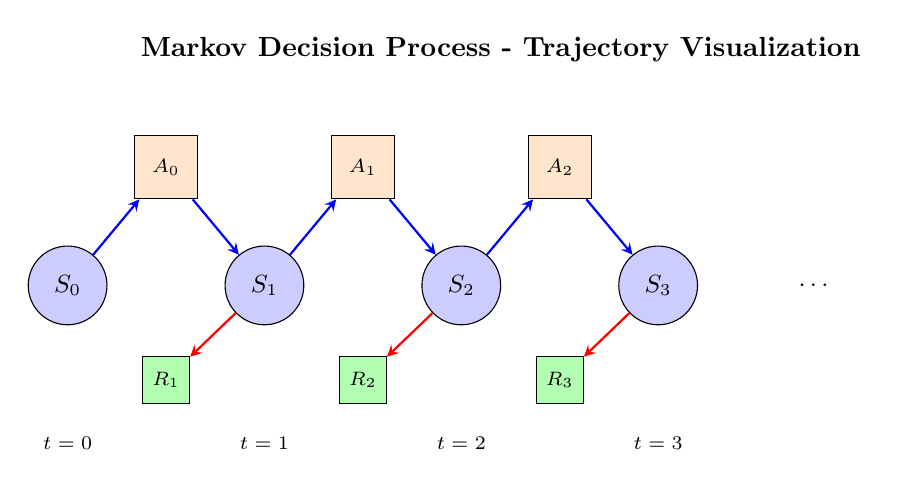
\begin{tikzpicture}[
    state/.style={circle, draw, fill=blue!20, minimum size=1cm, font=\small\bfseries},
    action/.style={rectangle, draw, fill=orange!20, minimum size=0.8cm, font=\scriptsize},
    reward/.style={rectangle, draw, fill=green!30, minimum size=0.6cm, font=\scriptsize},
    arrow/.style={->, >=stealth, thick}
]

% Title
\node[font=\bfseries] at (5.5, 3) {Markov Decision Process - Trajectory Visualization};

% States
\node[state] (s0) at (0, 0) {$S_0$};
\node[state] (s1) at (2.5, 0) {$S_1$};
\node[state] (s2) at (5, 0) {$S_2$};
\node[state] (s3) at (7.5, 0) {$S_3$};
\node[font=\small] at (9.5, 0) {$\cdots$};

% Actions
\node[action] (a0) at (1.25, 1.5) {$A_0$};
\node[action] (a1) at (3.75, 1.5) {$A_1$};
\node[action] (a2) at (6.25, 1.5) {$A_2$};

% Rewards
\node[reward] (r1) at (1.25, -1.2) {$R_1$};
\node[reward] (r2) at (3.75, -1.2) {$R_2$};
\node[reward] (r3) at (6.25, -1.2) {$R_3$};

% Arrows
\draw[arrow, blue] (s0) -- (a0);
\draw[arrow, blue] (a0) -- (s1);
\draw[arrow, blue] (s1) -- (a1);
\draw[arrow, blue] (a1) -- (s2);
\draw[arrow, blue] (s2) -- (a2);
\draw[arrow, blue] (a2) -- (s3);

\draw[arrow, red] (s1) -- (r1);
\draw[arrow, red] (s2) -- (r2);
\draw[arrow, red] (s3) -- (r3);

% Time labels
\node[font=\scriptsize] at (0, -2) {$t=0$};
\node[font=\scriptsize] at (2.5, -2) {$t=1$};
\node[font=\scriptsize] at (5, -2) {$t=2$};
\node[font=\scriptsize] at (7.5, -2) {$t=3$};

\end{tikzpicture}
\end{center}

\begin{tcolorbox}[colback=yellow!5!white,colframe=yellow!75!black,title=\textbf{The Credit Assignment Problem}]
In Full RL, rewards may be delayed many steps after the actions that caused them. This creates the \textbf{credit assignment problem}: how to attribute success/failure to individual actions?

\textbf{Example}: In chess, a brilliant opening move might contribute to a win 50 moves later. The agent must propagate credit backward through time.

\textbf{Mathematical Formulation}: The return $G_t$ incorporates all future rewards, weighted by discount factor:
\[
G_t = \underbrace{R_{t+1}}_{\text{immediate}} + \underbrace{\gamma R_{t+2} + \gamma^2 R_{t+3} + \ldots}_{\text{delayed}}
\]

TD learning and Monte Carlo methods differ in how they solve credit assignment:
\begin{itemize}
    \item \textbf{Monte Carlo}: Wait until episode ends, then assign full return to all visited states
    \item \textbf{TD Learning}: Use bootstrapping --- estimate credit immediately based on next state's value
\end{itemize}
\end{tcolorbox}

\subsection{Goals and Rewards}

The \textbf{Reward Hypothesis} (Sutton \& Barto): ``All of what we mean by goals and purposes can be well thought of as the maximisation of the expected value of the cumulative sum of a received scalar signal (reward).''

Characteristics of a good reward signal:
\begin{itemize}
    \item \textbf{Scalar}: A single number --- simple for learning algorithms to process.
    \item \textbf{Outside Agent's Control}: The agent cannot manipulate the reward signal itself. Forces honest behavior.
    \item \textbf{Bounded}: Rewards are finite. Prevents value estimates from diverging to $\pm\infty$.
\end{itemize}

The reward signal tells the agent \textbf{what} to achieve, not \textbf{how}. The agent must discover effective behavior on its own.

\subsection{Returns and Discounting}

The agent seeks to maximize the expected \textbf{return} $G_t$.

For \textbf{episodic tasks} (finite horizon $T$):
\[
G_t = R_{t+1} + R_{t+2} + R_{t+3} + \ldots + R_T
\]

For \textbf{continuing tasks} (infinite horizon):
\[
G_t = R_{t+1} + \gamma R_{t+2} + \gamma^2 R_{t+3} + \ldots = \sum_{k=0}^{\infty} \gamma^k R_{t+k+1}
\]

where $\gamma \in [0, 1]$ is the \textbf{discount factor}.

Key properties:
\begin{itemize}
    \item $\gamma = 0$: Myopic agent --- only cares about immediate reward $R_{t+1}$.
    \item $\gamma \to 1$: Farsighted agent --- treats distant future rewards almost as valuable as immediate ones.
    \item $\gamma < 1$ guarantees convergence of the infinite sum if rewards are bounded.
\end{itemize}

A useful recursive identity:
\[
G_t = R_{t+1} + \gamma G_{t+1}
\]

\subsubsection{Unified Notation}

Using the \textbf{absorbing state trick}: model episode termination as entering a special absorbing state that only transitions to itself with $R = 0$. Now both episodic and continuing tasks use the same formula:
\[
G_t = \sum_{k=0}^{\infty} \gamma^k R_{t+k+1}
\]

with the constraint that we cannot have both $T = \infty$ and $\gamma = 1$ simultaneously (otherwise the sum diverges).

\subsection{The Markov Property}

The \textbf{Markov property} is the foundation of RL state representation:
\[
P(S_{t+1} | S_t, A_t) = P(S_{t+1} | S_0, A_0, \ldots, S_t, A_t)
\]

In words: ``The future is independent of the past, given the present.'' The next state depends \textbf{only} on the current state and action. The full history before time $t$ is irrelevant if $S_t$ summarizes everything needed.

This allows algorithms to use \textbf{one-step transitions} for learning --- no need to store and process the full history of past states.

If the state does not capture enough information, the Markov property fails, leading to \textbf{Partially Observable MDPs (POMDPs)}.

\subsection{Episodic vs Continuing Tasks}

\textbf{Episodic tasks} naturally break into episodes --- finite sequences that each end at a terminal state, after which the environment resets. Examples: chess games, maze solving attempts, pole balancing episodes.

\textbf{Continuing tasks} have no terminal state. The agent--environment interaction goes on indefinitely. Examples: personal assistant robots, process control in factories. Rewards must be discounted to keep the return finite.

\subsection{State Value Function $V_\pi(s)$}

The \textbf{state-value function} $v_\pi(s)$ gives the expected return when starting in state $s$ and following policy $\pi$ thereafter:
\[
v_\pi(s) = \mathbb{E}_\pi[G_t | S_t = s] = \mathbb{E}_\pi\left[\sum_{k=0}^{\infty} \gamma^k R_{t+k+1} \bigg| S_t = s\right]
\]

Key insight: ``The value of a state is not a fixed property of the state --- it is a property of the state AND the policy.'' The same state can have different values under different policies.

\subsection{Action Value Function $Q_\pi(s, a)$}

The \textbf{action-value function} $q_\pi(s, a)$ gives the expected return when starting in state $s$, taking action $a$, and thereafter following policy $\pi$:
\[
q_\pi(s, a) = \mathbb{E}_\pi[G_t | S_t = s, A_t = a] = \mathbb{E}_\pi\left[\sum_{k=0}^{\infty} \gamma^k R_{t+k+1} \bigg| S_t = s, A_t = a\right]
\]

\subsection{Relationship Between V and Q}

The fundamental relationship:
\[
V_\pi(s) = \sum_a \pi(a|s) \cdot Q_\pi(s, a)
\]

The state value is a \textbf{weighted average} of action values, where the weights are given by the policy probabilities. This means if we know $Q_\pi(s, a)$ for all actions, we can compute $V_\pi(s)$.

Conversely:
\[
Q_\pi(s, a) = \sum_{s'} P(s'|s, a) [r + \gamma V_\pi(s')]
\]

The action value depends on the immediate reward and the discounted value of the next state.

\begin{tcolorbox}[colback=blue!5!white,colframe=blue!75!black,title=\textbf{Worked Example 19: Computing $V(0)$ Under Different Policies}]
\textbf{Given}: A 2-state MDP. From state 0: going left gives $r = +1$; going right gives $r = +2$. Episode ends after one action. $\gamma = 1$. Fixed Q-values: $Q(0, \text{left}) = 1.0$, $Q(0, \text{right}) = 2.0$.

\textbf{Calculate}: $V(0)$ for four policies.

\textbf{Solution}:
Using $V_\pi(0) = \pi(\text{left}|0) \cdot Q(0,\text{left}) + \pi(\text{right}|0) \cdot Q(0,\text{right})$:

\begin{enumerate}
    \item \textbf{Always Left}: $\pi = [1.0, 0.0]$
    \[
    V(0) = 1.0(1.0) + 0.0(2.0) = 1.0
    \]
    \item \textbf{Always Right}: $\pi = [0.0, 1.0]$
    \[
    V(0) = 0.0(1.0) + 1.0(2.0) = 2.0
    \]
    \item \textbf{50/50}: $\pi = [0.5, 0.5]$
    \[
    V(0) = 0.5(1.0) + 0.5(2.0) = 0.5 + 1.0 = 1.5
    \]
    \item \textbf{20\% Left / 80\% Right}: $\pi = [0.2, 0.8]$
    \[
    V(0) = 0.2(1.0) + 0.8(2.0) = 0.2 + 1.6 = 1.8
    \]
\end{enumerate}

\textbf{Answer}: $V(0) = 1.0, 2.0, 1.5, 1.8$ for the four policies.

\textbf{Interpretation}: The value of state 0 changes purely based on the policy, even though the Q-values are fixed. The optimal policy is ``Always Right'' with $V(0) = 2.0$.
\end{tcolorbox}

\begin{tcolorbox}[colback=green!5!white,colframe=green!75!black,title=\textbf{Worked Example 20: Value Function with Future Consequences}]
\textbf{Given}: 4-state world: $0 \xrightarrow{\text{left}} 1$ ($r=+1$), $0 \xrightarrow{\text{right}} 2$ ($r=+2$), $2 \xrightarrow{\text{right}} 3$ ($r=-10$). No further transitions. $\gamma = 1$.

\textbf{Calculate}: Updated Q-values and $V(0)$ under each policy.

\textbf{Solution}:
\begin{enumerate}
    \item $Q(0, \text{left}) = +1.0$ (unchanged, ends at state 1)
    \item $Q(0, \text{right}) = +2 + (-10) = -8.0$ (goes to state 2, then penalty at state 3)
\end{enumerate}

Policies:
\begin{enumerate}
    \item Always Left: $V(0) = 1.0(-8.0) + 1.0(1.0) = 1.0$
    \item Always Right: $V(0) = 1.0(-8.0) = -8.0$
    \item 50/50: $V(0) = 0.5(1.0) + 0.5(-8.0) = 0.5 - 4.0 = -3.5$
    \item 20/80: $V(0) = 0.2(1.0) + 0.8(-8.0) = 0.2 - 6.4 = -6.2$
\end{enumerate}

\textbf{Answer}: Always Left now gives $V(0) = 1.0$ (best); Always Right gives $V(0) = -8.0$ (catastrophic).

\textbf{Key Insight}: Maximizing immediate reward can destroy long-term return. In the 2-state world, ``Always Right'' was optimal. In the 4-state world, it is catastrophic because the immediate $+2$ is followed by a $-10$ penalty. This is exactly why full RL is needed: TD-learning and Q-learning discover $Q(0,\text{right}) = -8$ by propagating future penalties backward in time.
\end{tcolorbox}

\begin{tcolorbox}[colback=green!5!white,colframe=green!75!black,title=\textbf{Worked Example 21: Discounted Return Calculation}]
\textbf{Given}: Episode rewards: $R_1 = 2$, $R_2 = 3$, $R_3 = 5$, $R_4 = 1$. $\gamma = 0.9$.

\textbf{Calculate}: Returns $G_0$, $G_1$, $G_2$, $G_3$.

\textbf{Solution}:
\begin{enumerate}
    \item $G_3 = R_4 = 1$
    \item $G_2 = R_3 + \gamma G_3 = 5 + 0.9(1) = 5.9$
    \item $G_1 = R_2 + \gamma G_2 = 3 + 0.9(5.9) = 3 + 5.31 = 8.31$
    \item $G_0 = R_1 + \gamma G_1 = 2 + 0.9(8.31) = 2 + 7.479 = 9.479$
\end{enumerate}

\textbf{Answer}: $G_0 = 9.48$, $G_1 = 8.31$, $G_2 = 5.9$, $G_3 = 1.0$

\textbf{Interpretation}: With $\gamma = 0.9$, distant rewards are weighted slightly less. If $\gamma = 0$, all returns would equal the immediate next reward. If $\gamma = 1$, $G_0 = 2+3+5+1 = 11$.
\end{tcolorbox}

\subsection{Bellman Equations}

The \textbf{Bellman equations} express values recursively --- $V$ and $Q$ are defined in terms of each other. They are the foundation of dynamic programming and reinforcement learning algorithms.

\subsubsection{Bellman Equation for $V_\pi$}

\[
v_\pi(s) = \sum_a \pi(a|s) \sum_{s'} P(s'|s, a) [r + \gamma v_\pi(s')]
\]

Meaning: The value of state $s$ equals the expected immediate reward plus the discounted value of the next state, averaged over all actions (weighted by $\pi$) and all possible next states.

\subsubsection{Bellman Equation for $Q_\pi$}

\[
q_\pi(s, a) = \sum_{s'} P(s'|s, a) [r + \gamma \sum_{a'} \pi(a'|s') q_\pi(s', a')]
\]

\subsubsection{Bellman Optimality Equations}

For the \textbf{optimal} value functions:
\[
v^*(s) = \max_a \sum_{s'} P(s'|s, a) [r + \gamma v^*(s')]
\]
\[
q^*(s, a) = \sum_{s'} P(s'|s, a) [r + \gamma \max_{a'} q^*(s', a')]
\]

The optimal policy is then:
\[
\pi^*(s) = \arg\max_a q^*(s, a)
\]

\begin{center}
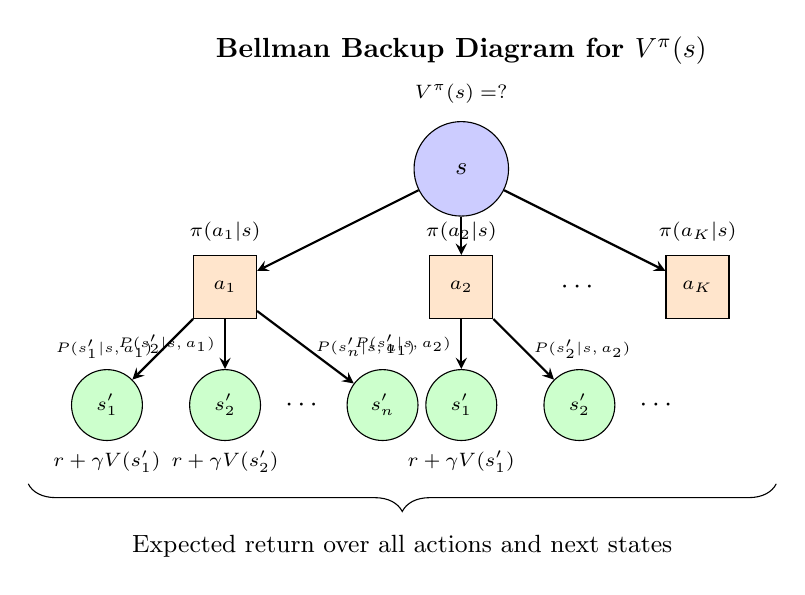
\begin{tikzpicture}[
    state/.style={circle, draw, fill=blue!20, minimum size=1.2cm, font=\small\bfseries},
    nextstate/.style={circle, draw, fill=green!20, minimum size=0.9cm, font=\scriptsize},
    action/.style={rectangle, draw, fill=orange!20, minimum size=0.8cm, font=\scriptsize},
    value/.style={rectangle, draw, fill=yellow!20, minimum size=0.7cm, font=\scriptsize},
    arrow/.style={->, >=stealth, thick}
]

% Title
\node[font=\bfseries] at (5, 5) {Bellman Backup Diagram for $V^\pi(s)$};

% Current state
\node[state] (s) at (5, 3.5) {$s$};
\node[above=0.1cm of s, font=\scriptsize] {$V^\pi(s) = ?$};

% Actions
\node[action] (a1) at (2, 2) {$a_1$};
\node[action] (a2) at (5, 2) {$a_2$};
\node[action] (ak) at (8, 2) {$a_K$};
\node at (6.5, 2) {$\cdots$};

% Policy probabilities
\node[font=\scriptsize] at (2, 2.7) {$\pi(a_1|s)$};
\node[font=\scriptsize] at (5, 2.7) {$\pi(a_2|s)$};
\node[font=\scriptsize] at (8, 2.7) {$\pi(a_K|s)$};

% Next states from a1
\node[nextstate] (s11) at (0.5, 0.5) {$s_1'$};
\node[nextstate] (s12) at (2, 0.5) {$s_2'$};
\node at (3, 0.5) {$\cdots$};
\node[nextstate] (s1n) at (4, 0.5) {$s_n'$};

% Next states from a2
\node[nextstate] (s21) at (5, 0.5) {$s_1'$};
\node[nextstate] (s22) at (6.5, 0.5) {$s_2'$};
\node at (7.5, 0.5) {$\cdots$};

% Arrows from s to actions
\draw[arrow] (s) -- (a1);
\draw[arrow] (s) -- (a2);
\draw[arrow] (s) -- (ak);

% Arrows from actions to next states
\draw[arrow] (a1) -- (s11) node[midway, left, font=\tiny] {$P(s_1'|s,a_1)$};
\draw[arrow] (a1) -- (s12) node[midway, left, font=\tiny] {$P(s_2'|s,a_1)$};
\draw[arrow] (a1) -- (s1n) node[midway, right, font=\tiny] {$P(s_n'|s,a_1)$};

\draw[arrow] (a2) -- (s21) node[midway, left, font=\tiny] {$P(s_1'|s,a_2)$};
\draw[arrow] (a2) -- (s22) node[midway, right, font=\tiny] {$P(s_2'|s,a_2)$};

% Value labels
\node[font=\scriptsize, below] at (s11.south) {$r + \gamma V(s_1')$};
\node[font=\scriptsize, below] at (s12.south) {$r + \gamma V(s_2')$};
\node[font=\scriptsize, below] at (s21.south) {$r + \gamma V(s_1')$};

% Curly brace showing expectation
\draw[decorate, decoration={brace, amplitude=10pt, mirror}] (-0.5, -0.5) -- (9, -0.5) node[midway, below=15pt, font=\small] {Expected return over all actions and next states};

\end{tikzpicture}
\end{center}

\begin{tcolorbox}[colback=yellow!5!white,colframe=yellow!75!black,title=\textbf{Bellman Equations: Theoretical Foundations}]
\textbf{Key Insight}: The Bellman equations encode the principle of \textbf{optimality} --- an optimal policy has the property that whatever the initial state and decision are, the remaining decisions must constitute an optimal policy with regard to the state resulting from the first decision (Bellman, 1957).

\textbf{Contraction Mapping}: The Bellman backup operator $\mathcal{T}^\pi$ is a \textbf{contraction} in the sup-norm:
\[
\|\mathcal{T}^\pi V - \mathcal{T}^\pi V'\|_\infty \leq \gamma \|V - V'\|_\infty
\]

This guarantees:
\begin{enumerate}
    \item \textbf{Unique solution}: There exists exactly one value function $v_\pi$ satisfying the Bellman equation
    \item \textbf{Convergence}: Iterative policy evaluation converges to $v_\pi$
    \item \textbf{Rate}: Convergence is geometric with factor $\gamma$
\end{enumerate}

\textbf{Proof Sketch}:
\begin{align}
    |\mathcal{T}^\pi V(s) - \mathcal{T}^\pi V'(s)| &= \left|\gamma \sum_{s'} P(s'|s,a) [V(s') - V'(s')]\right| \\
    &\leq \gamma \sum_{s'} P(s'|s,a) |V(s') - V'(s')| \\
    &\leq \gamma \|V - V'\|_\infty
\end{align}
\end{tcolorbox}

\begin{tcolorbox}[colback=green!5!white,colframe=green!75!black,title=\textbf{Worked Example: Bellman Operator Application}]
\textbf{Given}: A simple 2-state MDP with deterministic transitions. Policy: always go to the other state. $\gamma = 0.9$. Initial value guess: $V_0 = [0, 0]$.

\textbf{Apply the Bellman backup operator} $\mathcal{T}^\pi$:

\textbf{Iteration 1}:
\[
V_1(1) = r + \gamma V_0(2) = 1 + 0.9(0) = 1
\]
\[
V_1(2) = r + \gamma V_0(1) = 1 + 0.9(0) = 1
\]
Result: $V_1 = [1, 1]$

\textbf{Iteration 2}:
\[
V_2(1) = 1 + 0.9(1) = 1.9
\]
\[
V_2(2) = 1 + 0.9(1) = 1.9
\]
Result: $V_2 = [1.9, 1.9]$

\textbf{Iteration $k$}:
\[
V_k = \sum_{i=0}^{k-1} \gamma^i = \frac{1 - \gamma^k}{1 - \gamma}
\]

\textbf{Limit} ($k \to \infty$):
\[
V_\infty = \frac{1}{1 - \gamma} = \frac{1}{0.1} = 10
\]

This matches the analytical solution from the Bellman equation!
\end{tcolorbox}

\begin{tcolorbox}[colback=blue!5!white,colframe=blue!75!black,title=\textbf{Worked Example 22: Bellman Equation -- Recycling Robot}]
\textbf{Given}: A recycling robot with two energy levels: High (h) and Low (l). Actions: search (s), wait (w), recharge (re). Transitions:
\begin{itemize}
    \item Search when High: stays High with prob $\alpha$, becomes Low with prob $1-\alpha$
    \item Search when Low: stays Low with prob $\beta$, battery dies with prob $1-\beta$ (rescue required)
    \item Recharge: goes to High with probability 1
    \item Rewards: $r_s$ (search), $r_w$ (wait), $-3$ (rescue)
\end{itemize}

\textbf{Write}: Bellman optimality equations for $v^*(h)$ and $v^*(l)$.

\textbf{Solution}:
For state High:
\[
v^*(h) = \max \begin{cases}
r_s + \gamma[\alpha v^*(h) + (1-\alpha)v^*(l)] & \text{(search)} \\
r_w + \gamma v^*(h) & \text{(wait)}
\end{cases}
\]

For state Low:
\[
v^*(l) = \max \begin{cases}
r_s + \gamma[\beta v^*(l) + (1-\beta)(-3)] & \text{(search)} \\
r_w + \gamma v^*(l) & \text{(wait)} \\
\gamma v^*(h) & \text{(recharge)}
\end{cases}
\]

\textbf{Interpretation}: At each state, the optimal value is the maximum over all possible actions. Each action's value is the immediate reward plus the discounted expected value of the next state(s). The equations are coupled --- $v^*(h)$ depends on $v^*(l)$ and vice versa.
\end{tcolorbox}

\begin{tcolorbox}[colback=green!5!white,colframe=green!75!black,title=\textbf{Worked Example 23: Solving a Simple Bellman Equation}]
\textbf{Given}: A 2-state MDP with deterministic transitions. $r = +1$ for any transition. $\gamma = 0.9$. Policy: always go to the other state. Find $v_\pi(1)$ and $v_\pi(2)$.

\textbf{Solution}:
\begin{enumerate}
    \item $v_\pi(1) = 1 + \gamma v_\pi(2) = 1 + 0.9 v_\pi(2)$
    \item $v_\pi(2) = 1 + \gamma v_\pi(1) = 1 + 0.9 v_\pi(1)$
    \item Substitute (2) into (1): $v_\pi(1) = 1 + 0.9(1 + 0.9 v_\pi(1)) = 1 + 0.9 + 0.81 v_\pi(1)$
    \item $v_\pi(1) - 0.81 v_\pi(1) = 1.9$
    \item $0.19 v_\pi(1) = 1.9$
    \item $v_\pi(1) = \frac{1.9}{0.19} = 10.0$
    \item $v_\pi(2) = 1 + 0.9(10) = 1 + 9 = 10.0$
\end{enumerate}

\textbf{Answer}: $v_\pi(1) = 10.0$, $v_\pi(2) = 10.0$

\textbf{Interpretation}: Due to symmetry, both states have the same value. The high value (10) comes from the infinite horizon with positive rewards and $\gamma < 1$ ensuring convergence.
\end{tcolorbox}

\begin{tcolorbox}[colback=green!5!white,colframe=green!75!black,title=\textbf{Worked Example 24: Optimal Policy Selection from Q-Values}]
\textbf{Given}: Q-values at state $s$: $Q(s, a_1) = 5.2$, $Q(s, a_2) = 7.8$, $Q(s, a_3) = 3.1$.

\textbf{Calculate}: Optimal action and $V^*(s)$.

\textbf{Solution}:
\begin{enumerate}
    \item Optimal action: $\pi^*(s) = \arg\max_a Q(s, a) = a_2$ (since $7.8 > 5.2 > 3.1$)
    \item $V^*(s) = \max_a Q(s, a) = 7.8$
\end{enumerate}

\textbf{Answer}: $\pi^*(s) = a_2$, $V^*(s) = 7.8$

\textbf{Interpretation}: The optimal policy is greedy with respect to the optimal Q-function. This is why Q-learning is so powerful: once we learn $Q^*$, the optimal policy is trivial to extract.
\end{tcolorbox}


\section{Module 4: Dynamic Programming and Monte Carlo Methods}

\subsection{Dynamic Programming in RL}

Dynamic Programming (DP) refers to a collection of algorithms that can compute optimal policies for a Markov Decision Process (MDP) given a \textbf{perfect model} of the environment. A perfect model means both \textbf{transition probabilities} and \textbf{reward model} are known for the entire environment.

The key idea behind DP is the use of \textbf{value functions} to organize and structure the search for good policies. DP algorithms turn Bellman equations into \textbf{update rules} for improving approximations of the desired functions. DP contains two main steps:
\begin{enumerate}
    \item Break the problem into subproblems and solve each one.
    \item Cache or store solutions to subproblems for reuse to find the overall optimal solution.
\end{enumerate}

To solve a given MDP, we need to:
\begin{enumerate}
    \item Find out how good an arbitrary policy is (policy evaluation).
    \item Find out the optimal policy for the given MDP (policy improvement).
\end{enumerate}

\textbf{Limitations}:
\begin{itemize}
    \item Assumption of a perfect model is often unavailable for most real-world problems.
    \item Computational expense is very high --- it does not scale well as the number of states increases.
    \item However, DP is useful as a theoretical foundation on which most advanced RL methods are based.
\end{itemize}

\subsection{Policy Evaluation (Prediction)}

Policy evaluation computes the state-value function $v_\pi$ for an arbitrary policy $\pi$. Starting with some random initialization $v_0$, we iteratively update using the Bellman equation for $v_\pi$:
\[
v_{k+1}(s) = \sum_a \pi(a|s) \sum_{s', r} p(s', r | s, a)[r + \gamma v_k(s')]
\]

This is called \textbf{Iterative Policy Evaluation (IPE)}. Each sweep updates all states. The sequence $v_0, v_1, v_2, \ldots$ converges to $v_\pi$ as $k \to \infty$.

\subsubsection{Visual Gridworld Reference}

All gridworld examples use the standard 4$\times$4 gridworld (Sutton \& Barto). States 1--16 in row-major order. States 1 and 16 are terminal with $v=0$. All moves give $r=-1$. Actions \textbf{up}, \textbf{down}, \textbf{left}, \textbf{right} are deterministic; boundary moves keep the agent in place.

\begin{figure}[H]
\centering
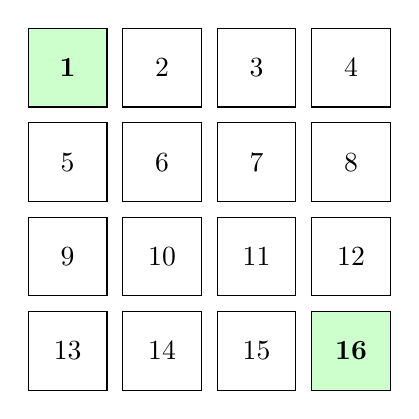
\begin{tikzpicture}[scale=1.2]
  \node[draw, fill=green!20, minimum size=1cm, font=\bfseries] (s1) at (0,3) {1};
  \node[draw, minimum size=1cm] (s2) at (1,3) {2};
  \node[draw, minimum size=1cm] (s3) at (2,3) {3};
  \node[draw, minimum size=1cm] (s4) at (3,3) {4};
  \node[draw, minimum size=1cm] (s5) at (0,2) {5};
  \node[draw, minimum size=1cm] (s6) at (1,2) {6};
  \node[draw, minimum size=1cm] (s7) at (2,2) {7};
  \node[draw, minimum size=1cm] (s8) at (3,2) {8};
  \node[draw, minimum size=1cm] (s9) at (0,1) {9};
  \node[draw, minimum size=1cm] (s10) at (1,1) {10};
  \node[draw, minimum size=1cm] (s11) at (2,1) {11};
  \node[draw, minimum size=1cm] (s12) at (3,1) {12};
  \node[draw, minimum size=1cm] (s13) at (0,0) {13};
  \node[draw, minimum size=1cm] (s14) at (1,0) {14};
  \node[draw, minimum size=1cm] (s15) at (2,0) {15};
  \node[draw, fill=green!20, minimum size=1cm, font=\bfseries] (s16) at (3,0) {16};
\end{tikzpicture}
\caption{Standard 4$\times$4 gridworld. Green cells are terminal (value 0). All moves incur $r=-1$.}
\label{fig:gridworld-layout}
\end{figure}

State 6 (center) is the focal state. Neighbors: up $\to$ 2, down $\to$ 10, left $\to$ 5, right $\to$ 7. The visual diagrams below overlay the Bellman backup onto this layout.

\begin{tcolorbox}[colback=blue!5!white,colframe=blue!75!black,title=\textbf{Worked Example 25: Gridworld Policy Evaluation}]
\textbf{Given}: A 4x4 gridworld with states numbered 1--16. States 1 and 16 are terminal (absorbing) with value 0. All other transitions give reward $r = -1$. Discount factor $\gamma = 1$. Actions: up, down, left, right (deterministic). Policy: \textbf{random} --- each action has probability 0.25. Compute $v_1$ for state 6.

\textbf{Solution}:
State 6 is surrounded by states 2 (up), 10 (down), 5 (left), 7 (right). All non-terminal.

For the random policy, each direction has probability 0.25. The Bellman update for state 6:
\[
v_1(6) = \sum_a \pi(a|6) \sum_{s'} p(s'|6, a)[r + \gamma v_0(s')]
\]

With $v_0(s) = 0$ for all non-terminal states and $v_0(1) = v_0(16) = 0$:
\begin{enumerate}
    \item Up (to state 2): $0.25 \times (-1 + 1 \cdot 0) = -0.25$
    \item Down (to state 10): $0.25 \times (-1 + 1 \cdot 0) = -0.25$
    \item Left (to state 5): $0.25 \times (-1 + 1 \cdot 0) = -0.25$
    \item Right (to state 7): $0.25 \times (-1 + 1 \cdot 0) = -0.25$
\end{enumerate}

\[
v_1(6) = -0.25 - 0.25 - 0.25 - 0.25 = -1.0
\]

\textbf{Answer}: $v_1(6) = -1.0$

\textbf{Visual Backup at State 6} ($v_0$ initialization):

\begin{center}
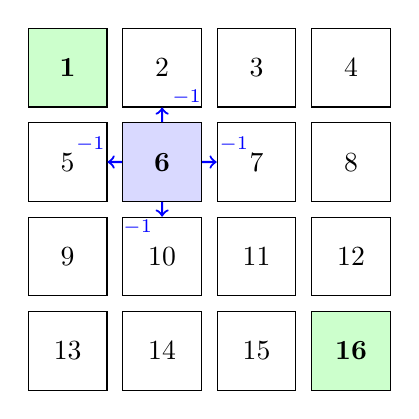
\begin{tikzpicture}[scale=1.2]
  \node[draw, fill=green!20, minimum size=1cm, font=\bfseries] (s1) at (0,3) {1};
  \node[draw, minimum size=1cm] (s2) at (1,3) {2};
  \node[draw, minimum size=1cm] (s3) at (2,3) {3};
  \node[draw, minimum size=1cm] (s4) at (3,3) {4};
  \node[draw, minimum size=1cm] (s5) at (0,2) {5};
  \node[draw, fill=blue!15, minimum size=1cm, font=\bfseries] (s6) at (1,2) {6};
  \node[draw, minimum size=1cm] (s7) at (2,2) {7};
  \node[draw, minimum size=1cm] (s8) at (3,2) {8};
  \node[draw, minimum size=1cm] (s9) at (0,1) {9};
  \node[draw, minimum size=1cm] (s10) at (1,1) {10};
  \node[draw, minimum size=1cm] (s11) at (2,1) {11};
  \node[draw, minimum size=1cm] (s12) at (3,1) {12};
  \node[draw, minimum size=1cm] (s13) at (0,0) {13};
  \node[draw, minimum size=1cm] (s14) at (1,0) {14};
  \node[draw, minimum size=1cm] (s15) at (2,0) {15};
  \node[draw, fill=green!20, minimum size=1cm, font=\bfseries] (s16) at (3,0) {16};
  \draw[->, thick, blue] (s6) -- (s2) node[midway, above right, font=\scriptsize] {$-1$};
  \draw[->, thick, blue] (s6) -- (s10) node[midway, below left, font=\scriptsize] {$-1$};
  \draw[->, thick, blue] (s6) -- (s5) node[midway, above left, font=\scriptsize] {$-1$};
  \draw[->, thick, blue] (s6) -- (s7) node[midway, above right, font=\scriptsize] {$-1$};
\end{tikzpicture}
\end{center}

State 6 receives four $-1$ rewards, each weighted 0.25.

Similarly, for all non-terminal states adjacent to non-terminal states: $v_1(s) = -1$.

For states adjacent to terminal states (e.g., state 2 adjacent to state 1):
\begin{itemize}
    \item Up (to state 1, terminal): $0.25 \times (-1 + 1 \cdot 0) = -0.25$
    \item Other directions: $-0.25$ each
    \item $v_1(2) = -1.0$ as well (all directions give $-1$ reward)
\end{itemize}

\textbf{Interpretation}: After one sweep, every non-terminal state has value $-1$, reflecting that any action incurs a $-1$ penalty. As sweeps continue, values propagate outward from the terminal states.
\end{tcolorbox}

\begin{tcolorbox}[colback=green!5!white,colframe=green!75!black,title=\textbf{Worked Example 26: Gridworld Second Sweep ($v_2$)}]
\textbf{Given}: Same gridworld. After first sweep, $v_1(s) = -1$ for all non-terminal states, $v_1(1) = v_1(16) = 0$. Compute $v_2(6)$.

\textbf{Solution}:
\begin{enumerate}
    \item Up (to state 2): $0.25 \times (-1 + 1 \cdot (-1)) = 0.25 \times (-2) = -0.5$
    \item Down (to state 10): $0.25 \times (-1 + (-1)) = -0.5$
    \item Left (to state 5): $0.25 \times (-1 + (-1)) = -0.5$
    \item Right (to state 7): $0.25 \times (-1 + (-1)) = -0.5$
\end{enumerate}

\[
v_2(6) = -0.5 - 0.5 - 0.5 - 0.5 = -2.0
\]

\textbf{Answer}: $v_2(6) = -2.0$

\textbf{Visual Value Map after Sweep 1} ($v_1$ in each cell):

\begin{center}
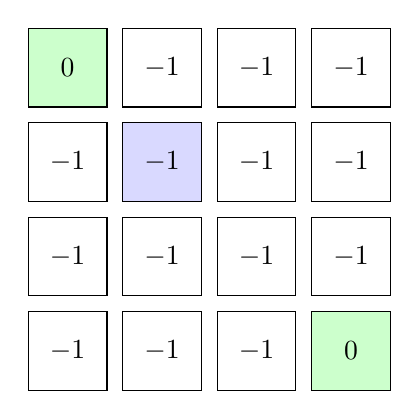
\begin{tikzpicture}[scale=1.2]
  \node[draw, fill=green!20, minimum size=1cm] at (0,3) {0};
  \node[draw, minimum size=1cm] at (1,3) {$-1$};
  \node[draw, minimum size=1cm] at (2,3) {$-1$};
  \node[draw, minimum size=1cm] at (3,3) {$-1$};
  \node[draw, minimum size=1cm] at (0,2) {$-1$};
  \node[draw, fill=blue!15, minimum size=1cm] at (1,2) {$-1$};
  \node[draw, minimum size=1cm] at (2,2) {$-1$};
  \node[draw, minimum size=1cm] at (3,2) {$-1$};
  \node[draw, minimum size=1cm] at (0,1) {$-1$};
  \node[draw, minimum size=1cm] at (1,1) {$-1$};
  \node[draw, minimum size=1cm] at (2,1) {$-1$};
  \node[draw, minimum size=1cm] at (3,1) {$-1$};
  \node[draw, minimum size=1cm] at (0,0) {$-1$};
  \node[draw, minimum size=1cm] at (1,0) {$-1$};
  \node[draw, minimum size=1cm] at (2,0) {$-1$};
  \node[draw, fill=green!20, minimum size=1cm] at (3,0) {0};
\end{tikzpicture}
\end{center}

The highlighted cell (state 6) is the focus. All non-terminal cells show $v_1 = -1$ because every move incurs $-1$ and neighbors still had $v_0 = 0$. Terminal cells remain 0 (green).

For states adjacent to terminal states, some directions lead to terminal (value 0):
\begin{itemize}
    \item $v_2(2)$: Up (terminal): $0.25(-1+0) = -0.25$; other 3 directions: $0.25(-1-1) = -0.5$ each
    \item $v_2(2) = -0.25 - 0.5 - 0.5 - 0.5 = -1.75$
\end{itemize}

\textbf{Interpretation}: Values propagate as negative distances from terminal states. After many sweeps, values converge to the expected number of steps to reach a terminal state.
\end{tcolorbox}

\begin{tcolorbox}[colback=green!5!white,colframe=green!75!black,title=\textbf{Worked Example 27: Value Iteration Step}]
\textbf{Given}: Same gridworld, but now with an \textbf{optimal} policy. We use value iteration (Bellman optimality backup). Compute $v_{k+1}(6)$ given $v_k(6) = -2$, $v_k(2) = v_k(10) = v_k(5) = v_k(7) = -2$.

\textbf{Solution}:
Value iteration takes the \textbf{maximum} over actions:
\[
v_{k+1}(6) = \max_a \sum_{s'} p(s'|6, a)[r + \gamma v_k(s')]
\]

For each action from state 6:
\begin{itemize}
    \item Up (to 2): $-1 + (-2) = -3$
    \item Down (to 10): $-1 + (-2) = -3$
    \item Left (to 5): $-1 + (-2) = -3$
    \item Right (to 7): $-1 + (-2) = -3$
\end{itemize}

All actions give $-3$, so the maximum is $-3$.

\textbf{Answer}: $v_{k+1}(6) = -3$

\textbf{Visual Value Iteration Step}: We take the \textbf{max} over actions. The diagram shows $v_k$ values (all $-2$); all neighbors are equal so every action yields $-3$. In later sweeps the max will point toward the nearest terminal.

\begin{center}
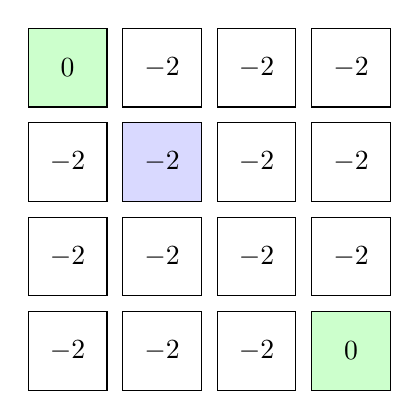
\begin{tikzpicture}[scale=1.2]
  \node[draw, fill=green!20, minimum size=1cm] at (0,3) {0};
  \node[draw, minimum size=1cm] at (1,3) {$-2$};
  \node[draw, minimum size=1cm] at (2,3) {$-2$};
  \node[draw, minimum size=1cm] at (3,3) {$-2$};
  \node[draw, minimum size=1cm] at (0,2) {$-2$};
  \node[draw, fill=blue!15, minimum size=1cm] at (1,2) {$-2$};
  \node[draw, minimum size=1cm] at (2,2) {$-2$};
  \node[draw, minimum size=1cm] at (3,2) {$-2$};
  \node[draw, minimum size=1cm] at (0,1) {$-2$};
  \node[draw, minimum size=1cm] at (1,1) {$-2$};
  \node[draw, minimum size=1cm] at (2,1) {$-2$};
  \node[draw, minimum size=1cm] at (3,1) {$-2$};
  \node[draw, minimum size=1cm] at (0,0) {$-2$};
  \node[draw, minimum size=1cm] at (1,0) {$-2$};
  \node[draw, minimum size=1cm] at (2,0) {$-2$};
  \node[draw, fill=green!20, minimum size=1cm] at (3,0) {0};
\end{tikzpicture}
\end{center}

\textbf{Interpretation}: In this symmetric case, all actions are equally bad. As values converge, the agent learns which paths lead to the nearest terminal state. Value iteration converges faster than full policy iteration because it combines evaluation and improvement in one step.
\end{tcolorbox}

\subsection{Policy Improvement}

Once we know $v_\pi$, we can improve the policy by making it greedy with respect to $v_\pi$. The new policy $\pi'$ selects at each state the action that maximizes the expected value:
\[
\pi'(s) = \arg\max_a \sum_{s', r} p(s', r | s, a)[r + \gamma v_\pi(s')]
\]

The \textbf{policy improvement theorem} guarantees that $\pi'$ is at least as good as $\pi$, and strictly better if any action is strictly better than $\pi(s)$.

\subsection{Policy Iteration}

\textbf{Policy iteration} alternates between policy evaluation and policy improvement:
\[
\pi_0 \xrightarrow{E} v_{\pi_0} \xrightarrow{I} \pi_1 \xrightarrow{E} v_{\pi_1} \xrightarrow{I} \pi_2 \xrightarrow{E} \cdots \xrightarrow{I} \pi^*
\]

Each iteration is guaranteed to produce a policy that is at least as good as the previous one. Given enough iterations, it converges to the optimal policy $\pi^*$.

A drawback is that each policy evaluation step itself requires multiple sweeps through all states. \textbf{Value iteration} addresses this by stopping evaluation after just one sweep, combining evaluation and improvement into a single update.

\subsection{Value Iteration}

Value iteration directly applies the Bellman optimality equation as an update rule:
\[
v_{k+1}(s) = \max_a \sum_{s', r} p(s', r | s, a)[r + \gamma v_k(s')]
\]

This is identical to the Bellman update in policy evaluation, except we take the \textbf{maximum} over all actions instead of averaging over the policy. Once the updates are small enough (below a threshold $\theta$), we can extract the optimal policy by acting greedily with respect to the final value function.

\subsection{Bootstrapping}

\textbf{Bootstrapping} means estimating something based on another estimation. In DP methods such as value iteration and policy iteration, bootstrapping is used to update the value function of a state based on the \textbf{estimated value of successor states}. This allows for efficient calculation of the optimal value function and policy.

\subsection{Monte Carlo Methods}

Monte Carlo (MC) methods require only \textbf{experience} --- sample sequences of states, actions, and rewards from actual or simulated interaction with an environment. The name comes from the Monte Carlo casino --- randomness and chance are central to the method. The core idea: instead of computing something analytically, you run random experiments and average the results.

Key difference from DP: MC methods do \textbf{not} require a model of the environment. They learn directly from sampled episodes.

\subsubsection{Types of Monte Carlo Prediction}

\textbf{First-Visit Monte Carlo}: Estimates $V(s)$ as the average of returns following the \textbf{first visit} to state $s$ in each episode.

\textbf{Every-Visit Monte Carlo}: Estimates $V(s)$ as the average of returns following \textbf{every visit} to state $s$ in each episode.

\begin{tcolorbox}[colback=blue!5!white,colframe=blue!75!black,title=\textbf{Worked Example 28: First-Visit vs Every-Visit MC}]
\textbf{Given}: Two episodes:
\begin{itemize}
    \item Episode 1: $A \xrightarrow{+3} A \xrightarrow{+2} B \xrightarrow{-4} B \xrightarrow{+4} A \xrightarrow{-3}$ (terminate)
    \item Episode 2: $A \xrightarrow{+3} B \xrightarrow{-2} B \xrightarrow{+3} A \xrightarrow{-3}$ (terminate)
\end{itemize}

\textbf{Calculate}: $V(A)$ and $V(B)$ using First-Visit and Every-Visit MC. $\gamma = 1$.

\textbf{Solution} --- First-Visit MC:
\begin{enumerate}
    \item \textbf{For $V(A)$}:
    \begin{itemize}
        \item Episode 1, first visit to A: return = $3 + 2 - 4 + 4 - 3 = 2$
        \item Episode 2, first visit to A: return = $3 - 2 + 3 - 3 = 1$
        \item $V(A) = \frac{2 + 1}{2} = 1.5$
    \end{itemize}
    \item \textbf{For $V(B)$}:
    \begin{itemize}
        \item Episode 1, first visit to B: return = $-4 + 4 - 3 = -3$
        \item Episode 2, first visit to B: return = $-2 + 3 - 3 = -2$
        \item $V(B) = \frac{-3 + (-2)}{2} = -2.5$
    \end{itemize}
\end{enumerate}

\textbf{Solution} --- Every-Visit MC:
\begin{enumerate}
    \item \textbf{For $V(A)$}:
    \begin{itemize}
        \item Episode 1 visits to A: first A gives $3+2-4+4-3 = 2$; second A gives $4-3 = 1$
        \item Episode 2 visits to A: first A gives $3-2+3-3 = 1$
        \item $V(A) = \frac{2 + 1 + 1}{3} = \frac{4}{3} \approx 1.33$
    \end{itemize}
    \item \textbf{For $V(B)$}:
    \begin{itemize}
        \item Episode 1 visits to B: first B gives $-4+4-3 = -3$; second B gives $-3$
        \item Episode 2 visits to B: first B gives $-2+3-3 = -2$; second B gives $-3$
        \item $V(B) = \frac{-3 + (-3) + (-2) + (-3)}{4} = \frac{-11}{4} = -2.75$
    \end{itemize}
\end{enumerate}

\textbf{Answer}:
\begin{center}
\begin{tabular}{|c|c|c|}
\hline
& First-Visit & Every-Visit \\ \hline
$V(A)$ & 1.5 & 1.33 \\ \hline
$V(B)$ & -2.5 & -2.75 \\ \hline
\end{tabular}
\end{center}

\textbf{Interpretation}: First-Visit and Every-Visit give different estimates. In the limit of infinite episodes, both converge to the true value. First-Visit is unbiased; Every-Visit is biased in finite samples but still consistent. For Blackjack (where states never repeat within an episode), both methods are identical.
\end{tcolorbox}

\begin{tcolorbox}[colback=green!5!white,colframe=green!75!black,title=\textbf{Worked Example 29: Monte Carlo Control}]
\textbf{Given}: Two episodes with exploring starts. After episode 1, $Q(s_1, a_1) = 5$ (1 sample). Episode 2 visits $(s_1, a_1)$ with return $G = 7$.

\textbf{Calculate}: Updated $Q(s_1, a_1)$ using incremental MC update. $\alpha = 0.1$.

\textbf{Solution}:
\begin{enumerate}
    \item First-visit count for $(s_1, a_1)$ becomes 2.
    \item Incremental update: $Q_{\text{new}} = Q_{\text{old}} + \frac{1}{N}(G - Q_{\text{old}})$
    \item $Q_{\text{new}} = 5 + \frac{1}{2}(7 - 5) = 5 + 1 = 6$
\end{enumerate}

Or with constant step-size: $Q_{\text{new}} = 5 + 0.1(7 - 5) = 5 + 0.2 = 5.2$

\textbf{Answer}: $Q = 6$ (sample average) or $Q = 5.2$ (constant step-size)

\textbf{Interpretation}: Sample average converges to the true mean. Constant step-size adapts faster to non-stationary environments but never fully converges --- it keeps oscillating around the true value.
\end{tcolorbox}

\begin{tcolorbox}[colback=green!5!white,colframe=green!75!black,title=\textbf{Worked Example 30: Blackjack State Value}]
\textbf{Given}: In Blackjack, the state is (player sum, dealer showing, usable ace). Consider the policy: stick if sum is 20 or 21, otherwise hit. After 1000 episodes, the average return following state (sum=18, dealer=7, no ace) is $-0.15$.

\textbf{Calculate}: $V(\text{sum}=18, \text{dealer}=7, \text{no ace})$.

\textbf{Solution}:
\begin{enumerate}
    \item Under first-visit MC: average of returns from first visits to this state across all episodes.
    \item $V = -0.15$
\end{enumerate}

\textbf{Answer}: $V = -0.15$

\textbf{Interpretation}: A slightly negative value indicates this state is slightly unfavorable under the current policy. The player is likely to bust or get a low final sum. Monte Carlo averages over the stochasticity of card draws, giving a reliable estimate given enough samples.
\end{tcolorbox}

\subsection{On-Policy vs Off-Policy Learning}

\textbf{On-Policy learning}: The algorithm evaluates and improves the \textbf{same} policy that is being used to select actions. Examples: Policy Iteration, Value Iteration, SARSA.

\textbf{Off-Policy learning}: The agent learns the value of a \textbf{target policy} $\pi$ while following a separate \textbf{behavior policy} $b$ for exploration. This allows continuous exploration while learning the optimal policy. Examples: Q-Learning.

Benefits of off-policy methods:
\begin{itemize}
    \item \textbf{Continuous exploration}: The behavior policy can keep exploring while the target policy converges to optimal.
    \item \textbf{Learning from demonstration}: Can learn from human demonstrations or other agents.
    \item \textbf{Parallel learning}: Multiple behavior policies can generate data for a single target policy.
\end{itemize}


\section{Module 5: Temporal Difference Learning}

\subsection{What is Temporal Difference Learning?}

\textbf{Temporal Difference (TD) learning} is a foundational class of algorithms in reinforcement learning that combine ideas from \textbf{Monte Carlo} methods and \textbf{Dynamic Programming}. Like MC, TD learns directly from raw experience without a model. Like DP, TD \textbf{bootstraps} --- updates guesses based on other guesses.

The key TD learning algorithm is \textbf{TD(0)}, which updates the value function after every step using the observed reward and the estimated value of the next state:
\[
V(S_t) \leftarrow V(S_t) + \alpha [R_{t+1} + \gamma V(S_{t+1}) - V(S_t)]
\]

The term $\delta_t = R_{t+1} + \gamma V(S_{t+1}) - V(S_t)$ is called the \textbf{TD error}. It represents the difference between:
\begin{itemize}
    \item The \textbf{bootstrap estimate} of the return: $R_{t+1} + \gamma V(S_{t+1})$ --- ``what I think the return is, based on immediate reward plus discounted estimate of next state''
    \item The \textbf{current estimate}: $V(S_t)$ --- ``what I currently believe this state's value is''
\end{itemize}

If $\delta_t > 0$, the outcome was better than expected --- we should \textbf{increase} $V(S_t)$. If $\delta_t < 0$, the outcome was worse than expected --- we should \textbf{decrease} $V(S_t)$. The learning rate $\alpha$ controls how aggressively we update.

\textbf{Advantages of TD(0)}:
\begin{itemize}
    \item Online learning: updates after every step, unlike MC which waits for episode end.
    \item Works in continuing (non-episodic) environments.
    \item Usually converges faster than MC in practice.
\end{itemize}

\begin{tcolorbox}[colback=blue!5!white,colframe=blue!75!black,title=\textbf{Worked Example 31: TD(0) Update}]
\textbf{Given}: $\alpha = 0.1$, $\gamma = 0.9$. Current estimates: $V(S_1) = 5.0$, $V(S_2) = 7.0$. Agent takes action in $S_1$, receives $R_{t+1} = 2$, and transitions to $S_2$.

\textbf{Calculate}: Updated $V(S_1)$.

\textbf{Solution}:
\begin{enumerate}
    \item Compute TD target: $R_{t+1} + \gamma V(S_2) = 2 + 0.9(7.0) = 2 + 6.3 = 8.3$
    \item Compute TD error: $\delta_t = 8.3 - 5.0 = 3.3$
    \item Update: $V(S_1) = 5.0 + 0.1(3.3) = 5.0 + 0.33 = 5.33$
\end{enumerate}

\textbf{Answer}: $V(S_1) = 5.33$

\textbf{Interpretation}: The immediate reward plus the value of the next state (8.3) was higher than our current estimate (5.0), so we increased $V(S_1)$ toward the TD target. With more updates, $V(S_1)$ will converge to its true value.
\end{tcolorbox}

\begin{tcolorbox}[colback=green!5!white,colframe=green!75!black,title=\textbf{Worked Example 32: TD(0) Negative Update}]
\textbf{Given}: $\alpha = 0.2$, $\gamma = 1.0$. Current: $V(A) = 10.0$, $V(B) = 8.0$, $V(C) = 5.0$. Agent moves $A \to B$ with $R = -1$, then $B \to C$ with $R = -2$.

\textbf{Calculate}: $V(A)$ and $V(B)$ after two TD(0) updates.

\textbf{Solution}:
\textbf{Step 1}: $A \to B$, $R = -1$
\begin{enumerate}
    \item TD target for A: $R + \gamma V(B) = -1 + 1.0(8.0) = 7.0$
    \item TD error: $\delta = 7.0 - 10.0 = -3.0$
    \item $V(A) = 10.0 + 0.2(-3.0) = 10.0 - 0.6 = 9.4$
\end{enumerate}

\textbf{Step 2}: $B \to C$, $R = -2$
\begin{enumerate}
    \item TD target for B: $R + \gamma V(C) = -2 + 1.0(5.0) = 3.0$
    \item TD error: $\delta = 3.0 - 8.0 = -5.0$
    \item $V(B) = 8.0 + 0.2(-5.0) = 8.0 - 1.0 = 7.0$
\end{enumerate}

\textbf{Answer}: $V(A) = 9.4$, $V(B) = 7.0$

\textbf{Interpretation}: Both states were overestimated. The negative rewards and lower-valued successor states caused the TD errors to be negative, reducing the value estimates. With more episodes, these estimates converge to the true expected returns.
\end{tcolorbox}

\begin{tcolorbox}[colback=green!5!white,colframe=green!75!black,title=\textbf{Worked Example 33: TD(0) Over Multiple Episodes}]
\textbf{Given}: A 2-state MDP: Start $\to$ A ($R=0$) $\to$ B ($R=10$), then terminate. $\gamma = 0.9$, $\alpha = 0.5$. Initial: $V(A) = 0$, $V(B) = 0$.

Episode 1: returns 10 at B. Episode 2: same. Episode 3: same.

\textbf{Calculate}: $V(A)$ and $V(B)$ after 3 episodes.

\textbf{Solution}:
\textbf{Episode 1}:
\begin{enumerate}
    \item $A \to B$: TD target = $0 + 0.9(0) = 0$, error = $0 - 0 = 0$. $V(A) = 0$.
    \item $B \to$ terminal: TD target = $10 + 0.9(0) = 10$, error = $10 - 0 = 10$. $V(B) = 0 + 0.5(10) = 5$.
\end{enumerate}

\textbf{Episode 2}:
\begin{enumerate}
    \item $A \to B$: TD target = $0 + 0.9(5) = 4.5$, error = $4.5 - 0 = 4.5$. $V(A) = 0 + 0.5(4.5) = 2.25$.
    \item $B \to$ terminal: TD target = $10 + 0 = 10$, error = $10 - 5 = 5$. $V(B) = 5 + 0.5(5) = 7.5$.
\end{enumerate}

\textbf{Episode 3}:
\begin{enumerate}
    \item $A \to B$: TD target = $0 + 0.9(7.5) = 6.75$, error = $6.75 - 2.25 = 4.5$. $V(A) = 2.25 + 0.5(4.5) = 4.5$.
    \item $B \to$ terminal: TD target = $10$, error = $10 - 7.5 = 2.5$. $V(B) = 7.5 + 0.5(2.5) = 8.75$.
\end{enumerate}

\textbf{Answer}: After 3 episodes: $V(A) = 4.5$, $V(B) = 8.75$

\textbf{Interpretation}: $V(B)$ converges toward 10 (the true terminal reward). $V(A)$ converges toward $0.9 \times 10 = 9$ (the discounted reward from reaching B). TD bootstraps --- $V(A)$ improves as $V(B)$ improves, even without reaching the terminal state.
\end{tcolorbox}

\subsection{On-Policy vs Off-Policy TD Control}

\textbf{On-policy}: Learn about the policy being followed (behavior policy = target policy). The agent explores and learns the same policy simultaneously. \textbf{SARSA} is an on-policy TD control algorithm.

\textbf{Off-policy}: Learn about a policy different from the one being followed (behavior policy $\neq$ target policy). The agent explores with one policy but learns the optimal target policy. \textbf{Q-Learning} is an off-policy TD control algorithm.

\subsection{SARSA: On-Policy TD Control}

SARSA updates the Q-value after every transition $S_t, A_t, R_{t+1}, S_{t+1}, A_{t+1}$ --- hence the name SARSA. The update rule:
\[
Q(S_t, A_t) \leftarrow Q(S_t, A_t) + \alpha [R_{t+1} + \gamma Q(S_{t+1}, A_{t+1}) - Q(S_t, A_t)]
\]

The next action $A_{t+1}$ is selected using the \textbf{current} policy (e.g., $\epsilon$-greedy with respect to current Q). This makes SARSA \textbf{on-policy}.

\begin{tcolorbox}[colback=blue!5!white,colframe=blue!75!black,title=\textbf{Worked Example 34: SARSA Update}]
\textbf{Given}: $\alpha = 0.5$, $\gamma = 1.0$. Q-table:
\begin{center}
\begin{tabular}{|c|c|c|c|}
\hline
& Left & Right & Up \\ \hline
A & 2.0 & 1.0 & 0.5 \\ \hline
B & 1.5 & 3.0 & 2.0 \\ \hline
C & 0.5 & 1.0 & 2.5 \\ \hline
\end{tabular}
\end{center}

Agent in state A takes action Right, gets $R = 5$, moves to B. In state B, uses greedy action (Up, $Q = 2.0$).

\textbf{Calculate}: Updated $Q(A, \text{Right})$.

\textbf{Solution}:
\begin{enumerate}
    \item Current $Q(A, \text{Right}) = 1.0$
    \item SARSA target: $R + \gamma Q(B, \text{Up}) = 5 + 1.0(2.0) = 7.0$
    \item TD error: $7.0 - 1.0 = 6.0$
    \item Update: $Q(A, \text{Right}) = 1.0 + 0.5(6.0) = 1.0 + 3.0 = 4.0$
\end{enumerate}

\textbf{Answer}: $Q(A, \text{Right}) = 4.0$

\textbf{Interpretation}: The transition from A to B via Right was very rewarding (immediate reward 5 + future value 2). SARSA updates $Q(A, \text{Right})$ aggressively toward this target.
\end{tcolorbox}

\begin{tcolorbox}[colback=green!5!white,colframe=green!75!black,title=\textbf{Worked Example 35: SARSA With Exploration}]
\textbf{Given}: Same Q-table as Example 34. $\epsilon = 0.1$. Agent in state A takes action Right (greedy), gets $R = 5$, moves to B. In B, $\epsilon$-greedy randomly selects Left ($Q = 1.5$) instead of greedy Up.

\textbf{Calculate}: Updated $Q(A, \text{Right})$.

\textbf{Solution}:
\begin{enumerate}
    \item Current $Q(A, \text{Right}) = 1.0$
    \item SARSA target: $R + \gamma Q(B, \text{Left}) = 5 + 1.0(1.5) = 6.5$
    \item TD error: $6.5 - 1.0 = 5.5$
    \item Update: $Q(A, \text{Right}) = 1.0 + 0.5(5.5) = 1.0 + 2.75 = 3.75$
\end{enumerate}

\textbf{Answer}: $Q(A, \text{Right}) = 3.75$

\textbf{Key Difference from Q-Learning}: SARSA uses the actual next action taken (Left, due to exploration), giving a target of 6.5. Q-Learning would use the maximum next Q-value (Up = 2.0), giving a target of 7.0. SARSA learns a more \textbf{conservative} policy that accounts for exploration mistakes.
\end{tcolorbox}

\begin{tcolorbox}[colback=green!5!white,colframe=green!75!black,title=\textbf{Worked Example 36: SARSA Episode Walkthrough}]
\textbf{Given}: A 2-state chain: A $\to$ B $\to$ terminal. Actions: only one action per state. $R(A) = 0$, $R(B) = 10$. $\gamma = 0.9$, $\alpha = 0.5$. Initial $Q(A) = 0$, $Q(B) = 0$.

\textbf{Episode}: A $\to$ B (R=0), B $\to$ terminal (R=10).

\textbf{Calculate}: Updated Q-values.

\textbf{Solution}:
\begin{enumerate}
    \item In A: target = $0 + 0.9 \cdot Q(B) = 0 + 0 = 0$. Error = $0 - 0 = 0$. $Q(A) = 0$.
    \item In B: target = $10 + 0 = 10$. Error = $10 - 0 = 10$. $Q(B) = 0 + 0.5(10) = 5$.
\end{enumerate}

After second episode (with updated $Q(B) = 5$):
\begin{enumerate}
    \item In A: target = $0 + 0.9(5) = 4.5$. Error = $4.5 - 0 = 4.5$. $Q(A) = 0 + 0.5(4.5) = 2.25$.
    \item In B: target = $10 + 0 = 10$. Error = $10 - 5 = 5$. $Q(B) = 5 + 0.5(5) = 7.5$.
\end{enumerate}

\textbf{Answer}: After 2 episodes: $Q(A) = 2.25$, $Q(B) = 7.5$

True values: $Q^*(B) = 10$, $Q^*(A) = 0.9 \times 10 = 9$. Converging toward these.
\end{tcolorbox}

\subsection{Q-Learning: Off-Policy TD Control}

Q-Learning updates Q-values using the \textbf{maximum} Q-value of the next state, regardless of which action was actually taken:
\[
Q(S_t, A_t) \leftarrow Q(S_t, A_t) + \alpha [R_{t+1} + \gamma \max_{a'} Q(S_{t+1}, a') - Q(S_t, A_t)]
\]

This is \textbf{off-policy} because the target uses $\max_{a'} Q(S_{t+1}, a')$ (the optimal action), while the behavior policy may explore randomly. Q-Learning learns the optimal policy directly, even while exploring.

\begin{tcolorbox}[colback=blue!5!white,colframe=blue!75!black,title=\textbf{Worked Example 37: Q-Learning Update}]
\textbf{Given}: Same Q-table as Example 34. $\alpha = 0.5$, $\gamma = 1.0$. Agent in state A takes action Right, gets $R = 5$, moves to B. In B, the actual action taken was Left, but Q-Learning uses the max.

\textbf{Calculate}: Updated $Q(A, \text{Right})$.

\textbf{Solution}:
\begin{enumerate}
    \item Current $Q(A, \text{Right}) = 1.0$
    \item $Q$-Learning target: $R + \gamma \max_{a'} Q(B, a') = 5 + 1.0 \times 3.0 = 8.0$ (max is Right = 3.0)
    \item TD error: $8.0 - 1.0 = 7.0$
    \item Update: $Q(A, \text{Right}) = 1.0 + 0.5(7.0) = 4.5$
\end{enumerate}

\textbf{Answer}: $Q(A, \text{Right}) = 4.5$

\textbf{Key Difference from SARSA}: Q-Learning target (8.0) $>$ SARSA target (6.5 or 7.0). Q-Learning is more \textbf{optimistic} because it assumes the best next action. It learns the optimal policy even while exploring suboptimally.
\end{tcolorbox}

\begin{tcolorbox}[colback=green!5!white,colframe=green!75!black,title=\textbf{Worked Example 38: Q-Learning vs SARSA Comparison}]
\textbf{Given}: A cliff-walking gridworld. States: A (start), B (cliff, reward -100), C (goal, reward +10). From A, action Right goes to C normally, but with 10\% chance falls to B.

\begin{center}
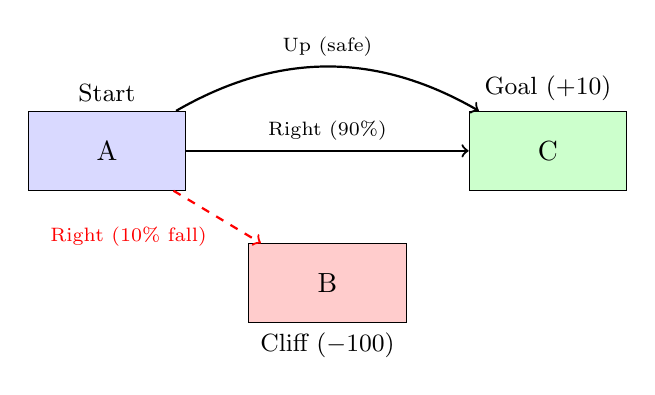
\begin{tikzpicture}[scale=1.4]
  \node[draw, fill=blue!15, minimum width=2cm, minimum height=1cm, label=above:{\small Start}] (A) at (0,0) {A};
  \node[draw, fill=red!20, minimum width=2cm, minimum height=1cm, label=below:{\small Cliff ($-100$)}] (B) at (2,-1.2) {B};
  \node[draw, fill=green!20, minimum width=2cm, minimum height=1cm, label=above:{\small Goal ($+10$)}] (C) at (4,0) {C};
  \draw[->, thick] (A) -- (C) node[midway, above, font=\scriptsize] {Right (90\%)};
  \draw[->, thick, red, dashed] (A) -- (B) node[midway, below left, font=\scriptsize] {Right (10\% fall)};
  \draw[->, thick, bend left=30] (A) to node[midway, above, font=\scriptsize] {Up (safe)} (C);
\end{tikzpicture}
\end{center}

Q-values: $Q(A, \text{Right}) = 5$, $Q(A, \text{Up}) = 4$. $\epsilon = 0.1$.

\textbf{Question}: Which algorithm (Q-Learning or SARSA) learns to take action Up to avoid the cliff?

\textbf{Solution}:
\begin{enumerate}
    \item \textbf{Q-Learning}: Updates using $\max$ next Q. Since the optimal path (Right without falling) has high value, Q-Learning learns $Q(A, \text{Right}) = 0.9(10) = 9$. But the behavior policy with $\epsilon = 0.1$ occasionally falls off the cliff.
    \item \textbf{SARSA}: Updates using the actual next action. Since 10\% of the time the agent falls (due to environment stochasticity or exploration), SARSA accounts for this risk. It learns a safer path (Up) with lower variance, even if the expected return is slightly lower.
\end{enumerate}

\textbf{Answer}: SARSA learns the safer policy (Up); Q-Learning learns the optimal policy (Right) but suffers from occasional falls during exploration.

\textbf{Interpretation}: Q-Learning is more \textbf{risk-seeking} (optimistic about future actions); SARSA is more \textbf{risk-averse} (considers actual behavior including exploration).
\end{tcolorbox}

\begin{tcolorbox}[colback=green!5!white,colframe=green!75!black,title=\textbf{Worked Example 39: Q-Learning Convergence}]
\textbf{Given}: A simple 3-state chain: S $\to$ A $\to$ G (goal). Only one action per state. $R(S \to A) = 0$, $R(A \to G) = 10$. $\gamma = 0.9$, $\alpha = 0.1$. Initial $Q = 0$ everywhere.

\textbf{After 100 episodes}: What are the converged Q-values?

\textbf{Solution}:
\begin{enumerate}
    \item $Q(G) = 0$ (terminal state)
    \item $Q(A) = R + \gamma \max Q(G) = 10 + 0 = 10$ (converged)
    \item $Q(S) = R + \gamma \max Q(A) = 0 + 0.9(10) = 9$ (converged)
\end{enumerate}

\textbf{Answer}: $Q(S) = 9.0$, $Q(A) = 10.0$, $Q(G) = 0$

\textbf{Interpretation}: Q-Learning converges to the optimal values by propagating rewards backward from the goal. The discount factor $\gamma = 0.9$ reduces the value of earlier states proportionally.
\end{tcolorbox}


\section{Module 6: Function Approximation and Deep Reinforcement Learning}

\subsection{Drawbacks of Tabular Methods}

Tabular methods (Q-tables, value tables) store an entry for every possible state (or state-action pair). This works well for small problems but suffers from major limitations:

\begin{itemize}
    \item \textbf{Large State Spaces}: A modest 10x10 grid with 4 actions has $100 \times 4 = 400$ entries. A video game with $84 \times 84$ grayscale pixels at 256 levels has $256^{7056}$ states --- completely intractable.
    \item \textbf{No Generalization}: In tabular methods, each state is treated independently. Changing the value of one state does not affect any other state, even if the states are very similar. This means the agent must visit every state many times to learn good values.
\end{itemize}

\textbf{Function approximation} solves both problems: instead of storing a table, we learn a \textbf{parameterized function} that maps states (or state-action pairs) to value estimates. This function can generalize across similar states and handle enormous state spaces.

\subsection{Value Function Approximation}

We approximate the value function $v_\pi$ (or action-value $q_\pi$) using a parameterized function:
\[
\hat{v}(s, \mathbf{w}) \approx v_\pi(s)
\]
where $\mathbf{w}$ is a vector of \textbf{weights} (parameters) learned through experience.

The goal is to minimize the \textbf{Mean Squared Value Error (MSVE)}:
\[
\text{MSVE}(\mathbf{w}) = \sum_{s \in \mathcal{S}} \mu(s) [v_\pi(s) - \hat{v}(s, \mathbf{w})]^2
\]
where $\mu(s)$ is a weighting factor (often the fraction of time spent in state $s$ under policy $\pi$).

\subsection{Gradient Descent Methods}

To optimize the weights, we use \textbf{gradient descent} (or ascent for maximization):
\[
\mathbf{w}_{t+1} = \mathbf{w}_t - \frac{1}{2} \alpha \nabla_w [v_\pi(S_t) - \hat{v}(S_t, \mathbf{w}_t)]^2
\]

Using stochastic gradient descent (SGD), we update weights after each sample:
\[
\mathbf{w}_{t+1} = \mathbf{w}_t + \alpha [v_\pi(S_t) - \hat{v}(S_t, \mathbf{w}_t)] \nabla_w \hat{v}(S_t, \mathbf{w}_t)
\]

\begin{tcolorbox}[colback=blue!5!white,colframe=blue!75!black,title=\textbf{Worked Example 40: Linear Parameterization Update}]
\textbf{Given}: A value function approximated as $\hat{v}(s, \mathbf{w}) = w_1 x_1(s) + w_2 x_2(s)$, where $\mathbf{x}(s) = [x_1, x_2]$ is the feature vector. Current weights: $\mathbf{w} = [2.0, -1.0]$. State $s$ has features $[3, 2]$. True return $v_\pi(s) = 5$. $\alpha = 0.1$.

\textbf{Calculate}: Updated weights.

\textbf{Solution}:
\begin{enumerate}
    \item Current estimate: $\hat{v}(s, \mathbf{w}) = 2.0(3) + (-1.0)(2) = 6 - 2 = 4$
    \item Prediction error: $v_\pi(s) - \hat{v} = 5 - 4 = 1$
    \item Gradients: $\nabla_w \hat{v} = [x_1, x_2] = [3, 2]$
    \item Update: $\Delta \mathbf{w} = \alpha \cdot \text{error} \cdot \nabla_w \hat{v} = 0.1(1)[3, 2] = [0.3, 0.2]$
    \item New weights: $\mathbf{w}_{\text{new}} = [2.0, -1.0] + [0.3, 0.2] = [2.3, -0.8]$
\end{enumerate}

\textbf{Verification}: New estimate = $2.3(3) + (-0.8)(2) = 6.9 - 1.6 = 5.3$, closer to 5.0.

\textbf{Answer}: $\mathbf{w}_{\text{new}} = [2.3, -0.8]$

\textbf{Interpretation}: The weight update moves the estimated value toward the target. Features with larger values ($x_1 = 3$) receive larger updates because they contribute more to the prediction.
\end{tcolorbox}

\begin{tcolorbox}[colback=green!5!white,colframe=green!75!black,title=\textbf{Worked Example 41: Feature Design for Function Approximation}]
\textbf{Given}: A gridworld agent at position $(x, y)$. We use linear FA with 3 features:
\begin{itemize}
    \item $f_1 = x$ (horizontal position)
    \item $f_2 = y$ (vertical position)
    \item $f_3 = \sqrt{x^2 + y^2}$ (distance from origin)
\end{itemize}

\begin{center}
\begin{tikzpicture}[scale=0.9]
  \draw[->] (0,0) -- (6,0) node[right] {$x$};
  \draw[->] (0,0) -- (0,6) node[above] {$y$};
  \foreach \i in {1,...,5} {
    \draw (\i,0.1) -- (\i,-0.1) node[below] {\i};
    \draw (0.1,\i) -- (-0.1,\i) node[left] {\i};
  }
  \fill[blue] (3,4) circle (4pt) node[above right, font=\small] {$(3,4)$};
  \draw[dashed, gray] (0,0) -- (3,4) node[midway, above left, font=\scriptsize] {$\sqrt{25}=5$};
\end{tikzpicture}
\end{center}

Weights: $w_1 = 1.0$, $w_2 = -0.5$, $w_3 = 2.0$. Compute $\hat{v}$ for state $(3, 4)$.

\textbf{Solution}:
\begin{enumerate}
    \item $f_1 = 3$, $f_2 = 4$, $f_3 = \sqrt{9 + 16} = \sqrt{25} = 5$
    \item $\hat{v} = 1.0(3) + (-0.5)(4) + 2.0(5) = 3 - 2 + 10 = 11$
\end{enumerate}

\textbf{Answer}: $\hat{v}(3, 4) = 11$

\textbf{Interpretation}: The value is a weighted sum of geometric features. This linear approximation generalizes to any $(x, y)$ position without requiring a separate table entry. However, the quality depends heavily on good feature design --- if the true value function is not well-approximated by these features, learning will be poor.
\end{tcolorbox}

\begin{tcolorbox}[colback=green!5!white,colframe=green!75!black,title=\textbf{Worked Example 42: Neural Network Value Estimation}]
\textbf{Given}: A neural network approximates $Q(s, a)$ with a single hidden layer. Input: 4-dimensional state vector. Hidden: 3 neurons with ReLU. Output: Q-value. Current weights produce $Q(s, a_1) = 5.2$, $Q(s, a_2) = 7.8$. Target (from TD): $R + \gamma \max Q(s', a') = 10$.

Learning rate $\alpha = 0.01$. Backpropagation computes $\frac{\partial Q}{\partial w}$ for each weight.

\textbf{Question}: How does the weight update differ from linear FA?

\textbf{Solution}:
\begin{enumerate}
    \item For the chosen action $a_2$: error = $10 - 7.8 = 2.2$
    \item Weight update: $\Delta w = \alpha \cdot \text{error} \cdot \frac{\partial Q}{\partial w} = 0.01(2.2) \nabla_w Q$
    \item Unlike linear FA where $\nabla_w \hat{v} = \mathbf{x}(s)$, neural networks have \textbf{nonlinear} gradients through ReLU and hidden layers.
    \item The gradient affects \textbf{all} weights in the network, not just the output layer weights for the active features.
\end{enumerate}

\textbf{Interpretation}: Neural networks can learn \textbf{arbitrary} feature representations automatically, unlike linear FA where features must be hand-designed. This is the core advantage of Deep RL.
\end{tcolorbox}

\subsection{Deep Q-Network (DQN)}

\textbf{DQN} combines Q-Learning with deep neural networks to approximate the action-value function $Q(s, a; \theta)$, where $\theta$ represents the neural network weights.

Key innovations of DQN:
\begin{enumerate}
    \item \textbf{Experience Replay}: Stores past transitions $(s, a, r, s')$ in a buffer and samples random mini-batches for training. This breaks correlation between consecutive samples and increases data efficiency.
    \item \textbf{Target Network}: Uses a separate network (with frozen weights, updated periodically) to compute TD targets. This stabilizes learning by preventing the moving target problem.
\end{enumerate}

The DQN loss function (Bellman update):
\[
L(\theta) = \mathbb{E} [(R + \gamma \max_{a'} Q(s', a'; \theta^-) - Q(s, a; \theta))^2]
\]
where $\theta^-$ are the frozen target network weights.

\subsection{Double DQN}

Standard DQN tends to \textbf{overestimate} Q-values because the same network selects and evaluates actions. \textbf{Double DQN} decouples these roles:
\begin{enumerate}
    \item Use the \textbf{online network} $Q(s', a'; \theta)$ to \textbf{select} the best action.
    \item Use the \textbf{target network} $Q(s', a'; \theta^-)$ to \textbf{evaluate} that action.
\end{enumerate}

The Double DQN update target:
\[
Y_t^{\text{DoubleDQN}} = R_{t+1} + \gamma Q(S_{t+1}, \arg\max_a Q(S_{t+1}, a; \theta_t); \theta_t^-)
\]

This reduces overestimation bias and often leads to more stable learning and better policies.

\subsection{Actor-Critic Architecture}

The \textbf{Actor-Critic} combines the benefits of policy-based and value-based methods:
\begin{itemize}
    \item \textbf{Actor}: A policy network $\pi(a|s; \theta)$ that selects actions.
    \item \textbf{Critic}: A value network $V(s; \mathbf{w})$ (or $Q(s,a; \mathbf{w})$) that evaluates the actions taken.
\end{itemize}

The critic provides a \textbf{baseline} that reduces the variance of policy gradient updates. The advantage function:
\[
A(s, a) = Q(s, a) - V(s)
\]
tells how much better action $a$ is compared to the average action in state $s$.

The actor updates using:
\[
\theta \leftarrow \theta + \alpha \nabla_\theta \log \pi(a|s; \theta) \cdot A(s, a)
\]

\subsection{A2C and A3C}

\textbf{A2C (Advantage Actor-Critic)}: Synchronous version where multiple workers collect experience in parallel but updates are applied centrally and synchronously.

\textbf{A3C (Asynchronous Advantage Actor-Critic)}: Multiple workers run in parallel on different CPU threads, each with its own copy of the environment. They compute gradients asynchronously and push them to a shared global network.

\subsection{DDPG and PPO}

\textbf{DDPG (Deep Deterministic Policy Gradient)} is designed for \textbf{continuous action spaces} (e.g., robotics, driving). It uses:
\begin{itemize}
    \item A deterministic actor $\mu(s)$ that outputs a continuous action directly.
    \item A critic $Q(s, a)$ that evaluates state-action pairs.
    \item Experience replay and target networks (similar to DQN).
\end{itemize}

\textbf{PPO (Proximal Policy Optimization)} is the most widely used RL algorithm today. It improves upon vanilla policy gradients by restricting policy updates to prevent large, destabilizing changes:

Define the probability ratio:
\[
r_t(\theta) = \frac{\pi_\theta(a_t | s_t)}{\pi_{\theta_{\text{old}}}(a_t | s_t)}
\]

The PPO objective with clipping:
\[
L^{\text{CLIP}}(\theta) = \mathbb{E}_t \left[ \min\left( r_t(\theta) \hat{A}_t, \; \text{clip}(r_t(\theta), 1 - \epsilon, 1 + \epsilon) \hat{A}_t \right) \right]
\]

where $\epsilon$ is a hyperparameter (typically 0.1 or 0.2).

\begin{tcolorbox}[colback=blue!5!white,colframe=blue!75!black,title=\textbf{Worked Example 43: PPO Clipping}]
\textbf{Given}: Advantage $\hat{A}_t = +5$ (good action). Old policy probability: $\pi_{\text{old}} = 0.3$. New policy probability: $\pi_\theta = 0.5$. $\epsilon = 0.2$.

\textbf{Calculate}: The clipped objective value.

\textbf{Solution}:
\begin{enumerate}
    \item Probability ratio: $r_t = \frac{0.5}{0.3} = 1.667$
    \item Clip range: $[1 - 0.2, 1 + 0.2] = [0.8, 1.2]$
    \item Since $r_t = 1.667 > 1.2$, the clipped ratio = $1.2$
    \item Unclipped term: $r_t \cdot \hat{A}_t = 1.667 \times 5 = 8.335$
    \item Clipped term: $\text{clip}(r_t) \cdot \hat{A}_t = 1.2 \times 5 = 6.0$
    \item Objective: $\min(8.335, 6.0) = 6.0$
\end{enumerate}

\textbf{Answer}: Objective = 6.0 (clipped version used because ratio exceeded $1+\epsilon$)

\textbf{Interpretation}: The new policy made action 67\% more likely than the old policy ($r_t = 1.667$), but PPO clips at 1.2 (20\% increase). The agent does not get extra reward for making the action \emph{too} much more likely, preventing overly aggressive updates that could destabilize training.
\end{tcolorbox}

\begin{tcolorbox}[colback=green!5!white,colframe=green!75!black,title=\textbf{Worked Example 44: PPO with Negative Advantage}]
\textbf{Given}: $\hat{A}_t = -4$ (bad action). $\pi_{\text{old}} = 0.4$. $\pi_\theta = 0.1$. $\epsilon = 0.2$.

\textbf{Calculate}: Clipped objective.

\textbf{Solution}:
\begin{enumerate}
    \item Probability ratio: $r_t = \frac{0.1}{0.4} = 0.25$
    \item Clip range: $[0.8, 1.2]$
    \item Since $r_t = 0.25 < 0.8$, the clipped ratio = $0.8$
    \item Unclipped term: $r_t \cdot \hat{A}_t = 0.25 \times (-4) = -1.0$
    \item Clipped term: $0.8 \times (-4) = -3.2$
    \item Objective: $\min(-1.0, -3.2) = -3.2$
\end{enumerate}

\textbf{Answer}: Objective = -3.2 (clipped version used because ratio fell below $1-\epsilon$)

\textbf{Interpretation}: For a bad action, PPO wants to decrease its probability. The new policy already decreased it significantly ($r_t = 0.25$, probability dropped to 1/4). But PPO limits the penalty to $0.8 \times (-4) = -3.2$, preventing the policy from completely abandoning the action too quickly.
\end{tcolorbox}

\begin{tcolorbox}[colback=green!5!white,colframe=green!75!black,title=\textbf{Worked Example 45: PPO Ratio Within Clip Range}]
\textbf{Given}: $\hat{A}_t = +3$. $\pi_{\text{old}} = 0.5$. $\pi_\theta = 0.55$. $\epsilon = 0.2$.

\textbf{Calculate}: Objective value.

\textbf{Solution}:
\begin{enumerate}
    \item Probability ratio: $r_t = \frac{0.55}{0.5} = 1.1$
    \item Clip range: $[0.8, 1.2]$
    \item Since $0.8 < 1.1 < 1.2$, ratio is within clip range
    \item Clipped ratio = $r_t = 1.1$ (no clipping)
    \item Objective: $r_t \cdot \hat{A}_t = 1.1 \times 3 = 3.3$
\end{enumerate}

\textbf{Answer}: Objective = 3.3 (unclipped, since ratio is within safe range)

\textbf{Interpretation}: When the policy change is moderate (10\% increase, within $\pm 20\%$), PPO allows full gradient updates. This ensures the policy improves without dangerous overshooting.
\end{tcolorbox}

\subsection{Algorithm Comparison Summary}

\begin{center}
\begin{tabular}{|l|l|l|l|l|}
\hline
\textbf{Algorithm} & \textbf{Type} & \textbf{Action Space} & \textbf{Learns} & \textbf{Key Trait} \\ \hline
DQN & Value-based & Discrete & $Q(s,a)$ & Replay buffer, target network \\ \hline
Double DQN & Value-based & Discrete & $Q(s,a)$ & Reduces overestimation \\ \hline
REINFORCE & Policy-based & Both & $\pi(a|s)$ & Monte Carlo, high variance \\ \hline
A2C & Actor-Critic & Both & $\pi + V$ & Synchronous parallel workers \\ \hline
A3C & Actor-Critic & Both & $\pi + V$ & Asynchronous parallel workers \\ \hline
DDPG & Actor-Critic & Continuous & $\mu(s) + Q$ & Replay buffer, deterministic \\ \hline
PPO & Actor-Critic & Both & $\pi + V$ & Clipped updates, most popular \\ \hline
\end{tabular}
\end{center}

\subsection{Prioritized Experience Replay}

In standard experience replay, transitions are sampled uniformly from the replay buffer. \textbf{Prioritized Experience Replay} samples transitions with probability proportional to their \textbf{TD error} magnitude:
\[
P(i) = \frac{|\delta_i|}{\sum_j |\delta_j|}
\]

Transitions with large TD errors (surprising outcomes) are sampled more frequently, making learning more efficient. A small constant $\epsilon$ is added to prevent zero probabilities for low-error transitions.

\end{document}
